% =====================================================================
%  Rapport complet -- Projet AVC
%  Segmentation des lésions d'AVC sur IRM T1 et domain shift inter-centres
%  Compilation : pdflatex rapport.tex (deux fois, pour la table des matières)
%  ou import direct du dossier dans Overleaf.
% =====================================================================
\documentclass[11pt,a4paper]{report}

% ---------- Langue et police ----------
\usepackage[utf8]{inputenc}
\usepackage[T1]{fontenc}
\usepackage[french]{babel}
\usepackage{lmodern}
\usepackage{microtype}

% ---------- Mise en page ----------
\usepackage[a4paper,margin=2.5cm]{geometry}
\usepackage{setspace}
\onehalfspacing
\usepackage{parskip}

% ---------- Tableaux, figures, maths ----------
\usepackage{graphicx}
\graphicspath{{figures/}}
\usepackage{booktabs}
\usepackage{tabularx}
\usepackage{array}
\usepackage{multirow}
\usepackage{float}
\usepackage{caption}
\captionsetup{font=small,labelfont=bf}
\usepackage{amsmath,amssymb}
\usepackage{enumitem}
\setlist{itemsep=2pt,topsep=4pt}

% ---------- Schémas ----------
\usepackage{tikz}
\usetikzlibrary{positioning,arrows.meta,calc,babel}

% ---------- Code et liens ----------
\usepackage{xcolor}
\usepackage{listings}
\lstset{basicstyle=\ttfamily\small,breaklines=true,frame=single,
        backgroundcolor=\color{gray!8},columns=fullflexible}
\usepackage[hidelinks]{hyperref}

% ---------- Raccourcis ----------
\newcommand{\fichier}[1]{\texttt{#1}}
\definecolor{accent}{RGB}{37,99,235}

% =====================================================================
\begin{document}

% ---------------------------------------------------------------------
%  Page de titre
% ---------------------------------------------------------------------
\begin{titlepage}
  \centering
  \vspace*{1.5cm}
  {\Large Projet de fin de module \par}
  \vspace{1.5cm}
  \rule{\linewidth}{0.6pt}\par\vspace{0.4cm}
  {\huge\bfseries Segmentation des lésions d'AVC sur IRM T1\\[0.3cm]
   et analyse du décalage inter-centres \par}
  \vspace{0.4cm}\rule{\linewidth}{0.6pt}\par
  \vspace{1.5cm}
  {\large Rapport complet du projet \par}
  \vspace{2cm}
  {\large
  \begin{tabular}{rl}
    \textbf{Équipe :} & Yosra Gadhgadhi \\
                      & Fayfa \\
                      & Anas \\[0.4cm]
    \textbf{Encadrant :} & \textit{(à compléter)} \\
  \end{tabular}\par}
  \vfill
  {\large Novembre 2026 \par}
\end{titlepage}

% ---------------------------------------------------------------------
%  Résumé
% ---------------------------------------------------------------------
\begin{abstract}
Ce projet segmente les lésions d'accident vasculaire cérébral (AVC) sur des
IRM T1 issues de 55 centres hospitaliers et mesure la perte de performance
lorsqu'un modèle est appliqué à un centre absent de l'entraînement
(\emph{domain shift}). Un pipeline Spark contrôle, réoriente, rééchantillonne
et normalise 1\,415 volumes, exportés avec une partition commune sans fuite :
916 cas d'entraînement en cinq plis, 231 cas de test ID et 268 cas de test OOD
issus de six centres entièrement retirés.

Le prétraitement réduit la distance relative médiane entre centres de 0,1315 à
0,0376 et fait passer la reconnaissance du centre à partir de l'histogramme
d'intensité de 69,7\,\% à 48,9\,\% d'exactitude équilibrée (hasard : 4\,\%).
Le centre reste donc identifiable. Sur un protocole historique, le meilleur
réseau (U-Net à encodeur ResNet-34 pré-entraîné) atteint un Dice de 0,47 en ID
et 0,53 en OOD : aucune baisse mesurable sur les centres inconnus, l'écart
s'expliquant par la taille des lésions. Des modules de généralisation
(augmentation, FDA, randomisation du style) et d'adaptation (DANN, TENT), une
démonstration web avec visualisation 3D et une suite de tests complètent le
travail. Les comparaisons finales sur la partition v2 attendent les modèles
entraînés.

\medskip
\noindent\textbf{Mots-clés :} AVC, segmentation, IRM, U-Net, nnU-Net,
généralisation de domaine, DANN, TENT, Spark.
\end{abstract}

\tableofcontents
\listoffigures
\listoftables

% =====================================================================
\chapter{Introduction}
% =====================================================================

\section{Contexte}

L'AVC est une cause majeure de handicap. La segmentation des lésions sur IRM
permet de mesurer leur volume et leur localisation, deux informations utiles
au pronostic et au suivi de la rééducation. Tracer ces lésions à la main est
long et variable d'un expert à l'autre ; les réseaux de neurones convolutifs
de type U-Net automatisent cette tâche.

Ces réseaux sont entraînés sur des images venant de quelques centres. Or les
centres diffèrent par leur scanner, leur protocole d'acquisition et leur
résolution. Ces différences modifient la distribution des intensités et
peuvent dégrader un modèle appliqué à un centre qu'il n'a jamais vu. Mesurer
ce décalage, puis l'anticiper et le réduire, est une condition pour un usage
clinique fiable.

\section{Objectifs et questions de recherche}

Le projet poursuit trois objectifs : construire un jeu de données propre et
une partition commune sans fuite ; mesurer le décalage entre centres ;
évaluer les méthodes qui le réduisent. Trois questions de recherche
structurent le travail :

\begin{description}
  \item[RQ1] Quel est l'écart de performance entre le test ID (centres vus à
  l'entraînement) et le test OOD (centres inconnus) ?
  \item[RQ2] Les architectures Transformer généralisent-elles mieux que
  nnU-Net ?
  \item[RQ3] Quelles techniques de généralisation (augmentation, DANN) ou
  d'adaptation au test (TENT) réduisent cet écart ?
\end{description}

\section{Organisation du projet et du rapport}

Le projet s'étend sur 14 semaines (tableau~\ref{tab:planning}). Le
chapitre~\ref{chap:etat} présente l'état de l'art, le
chapitre~\ref{chap:donnees} les données et le prétraitement, le
chapitre~\ref{chap:methodo} la méthodologie, le chapitre~\ref{chap:resultats}
les résultats. Les chapitres suivants décrivent la démonstration, la
validation, l'organisation de l'équipe, les limites et la conclusion.

\begin{table}[H]
  \centering
  \caption{Planning du projet.}
  \label{tab:planning}
  \begin{tabular}{ll}
    \toprule
    \textbf{Semaines} & \textbf{Livrable} \\
    \midrule
    S1--S2   & Exploration des données et contrôle qualité \\
    S3--S4   & Pipeline Spark, partitions et export nnU-Net \\
    S5--S6   & Statistiques avant/après et empreinte du centre \\
    S7--S10  & Analyses Dice, délai post-AVC et représentations \\
    S8--S12  & Démonstration Gradio, NiiVue, atlas et Docker \\
    S12--S14 & Rapport et soutenance \\
    \bottomrule
  \end{tabular}
\end{table}

% =====================================================================
\chapter{État de l'art}
\label{chap:etat}
% =====================================================================

\section{Segmentation des lésions d'AVC}

Le U-Net~\cite{ronneberger2015} associe un encodeur, qui réduit l'image et
extrait des caractéristiques, et un décodeur, qui la ramène à sa taille
d'origine ; des connexions directes transmettent les détails fins de
l'encodeur au décodeur. nnU-Net~\cite{isensee2021} configure
automatiquement le prétraitement, l'architecture et l'entraînement d'un
U-Net ; il sert de référence en segmentation médicale. Les architectures
Transformer, comme UNETR~\cite{hatamizadeh2022} et
Swin-UNETR~\cite{hatamizadeh2022swin}, modélisent des dépendances à longue
distance dans le volume.

Le jeu ATLAS~\cite{liew2018,liew2022} rassemble des IRM T1 de patients après
AVC, accompagnées de masques tracés manuellement, issues de nombreux centres.
Il est donc adapté à l'étude du décalage inter-centres.

\section{Généralisation et adaptation de domaine}

Les méthodes de \emph{généralisation} visent un modèle robuste à des centres
jamais vus, sans données de ces centres. BigAug~\cite{zhang2020} empile des
augmentations d'intensité, de qualité et de géométrie. FDA~\cite{yang2020}
remplace le spectre basse fréquence d'une image par celui d'une autre, ce qui
change son « style » sans toucher à l'anatomie. La randomisation du style
applique des convolutions aléatoires aux intensités.

Les méthodes d'\emph{adaptation} utilisent des données du domaine cible.
DANN~\cite{ganin2016} ajoute un classifieur de domaine relié à l'encodeur par
une couche d'inversion de gradient, pour que les caractéristiques ne
permettent plus de deviner le centre. TENT~\cite{wang2021} adapte un modèle
déjà entraîné au moment du test, sans étiquettes, en minimisant l'entropie
de ses prédictions.

\section{Mesure du décalage}

La distance de Wasserstein et la MMD (\emph{Maximum Mean
Discrepancy})~\cite{gretton2012} comparent deux distributions. Appliquées aux
histogrammes d'intensité ou aux représentations internes d'un réseau, elles
quantifient l'écart entre un centre et la référence d'entraînement.

\begin{table}[H]
  \centering
  \caption{Approches utilisées ou comparées dans le projet.}
  \label{tab:etat}
  \begin{tabularx}{\textwidth}{lXX}
    \toprule
    \textbf{Famille} & \textbf{Référence} & \textbf{Rôle dans le projet} \\
    \midrule
    Données          & ATLAS v2/v3~\cite{liew2018,liew2022} & 1\,453 IRM T1 multi-centres \\
    CNN              & U-Net~\cite{ronneberger2015} & Baselines (encodeur ResNet-34) \\
    CNN auto-configuré & nnU-Net~\cite{isensee2021} & Référence pour RQ2, export dédié \\
    Transformers     & UNETR, Swin-UNETR~\cite{hatamizadeh2022,hatamizadeh2022swin} & Comparés à nnU-Net (RQ2) \\
    Augmentation     & BigAug~\cite{zhang2020} & Généralisation sans données cibles (RQ3) \\
    Fourier          & FDA~\cite{yang2020} & Échange de style entre centres (RQ3) \\
    Adversarial      & DANN~\cite{ganin2016} & Effacer l'empreinte du centre (RQ3) \\
    Adaptation au test & TENT~\cite{wang2021} & Adapter les normalisations, sans étiquettes \\
    Distances        & Wasserstein, MMD~\cite{gretton2012} & Mesurer le décalage (S5) \\
    \bottomrule
  \end{tabularx}
\end{table}

% =====================================================================
\chapter{Données et prétraitement}
\label{chap:donnees}
% =====================================================================

Sur 1\,453 paires IRM/masque inventoriées dans 55 centres, 1\,415 cas de 54
centres sont prétraités, validés et exportés (livraison v2). Les 38 cas
exclus le sont avec un motif documenté.

\section{Jeu de données}

Les données proviennent d'ATLAS v3 / ISLES'26 : une IRM T1 et un masque
lésionnel manuel par patient, avec des métadonnées (centre, délai
post-AVC). L'archive est chiffrée et les données brutes restent privées ;
elles ne sont jamais versionnées.

\section{Exploration et contrôle qualité}

L'exploration des semaines 1 et 2 a relevé plusieurs pièges, tous traités par
le pipeline (tableau~\ref{tab:qc}).

\begin{table}[H]
  \centering
  \caption{Constats de l'exploration et décisions associées.}
  \label{tab:qc}
  \begin{tabularx}{\textwidth}{Xl}
    \toprule
    \textbf{Constat} & \textbf{Décision} \\
    \midrule
    R032 : espacement des voxels incohérent (cerveau de 31 cm), 37 cas & Exclu \\
    R065 : 1,76\,\% de la lésion hors du recadrage (tolérance 1\,\%), 1 cas & Quarantaine dans v2 \\
    R029 : fond à environ 0,0007 au lieu de 0 & Cerveau = intensité $>$ fond \\
    41 masques codés 0,99999998 & Seuillage \fichier{mask > 0.5} \\
    5 masques vides & Conservés comme cas négatifs \\
    Délai post-AVC absent ou invalide : 342 cas retenus (24,2\,\%) & Signalé, paire conservée \\
    \fichier{CHRONICITY} codé 1/vide & Non interprété comme un stade \\
    \bottomrule
  \end{tabularx}
\end{table}

La synthèse par centre (figure~\ref{fig:qc}) retrouve 1\,415 sujets retenus,
38 exclus et aucune erreur active. Huit centres retenus n'ont aucun délai
utilisable. Le drapeau \fichier{CHRONICITY} est renseigné pour 296 sujets
seulement ; son absence ne permet pas de déduire un stade clinique.

\begin{figure}[H]
  \centering
  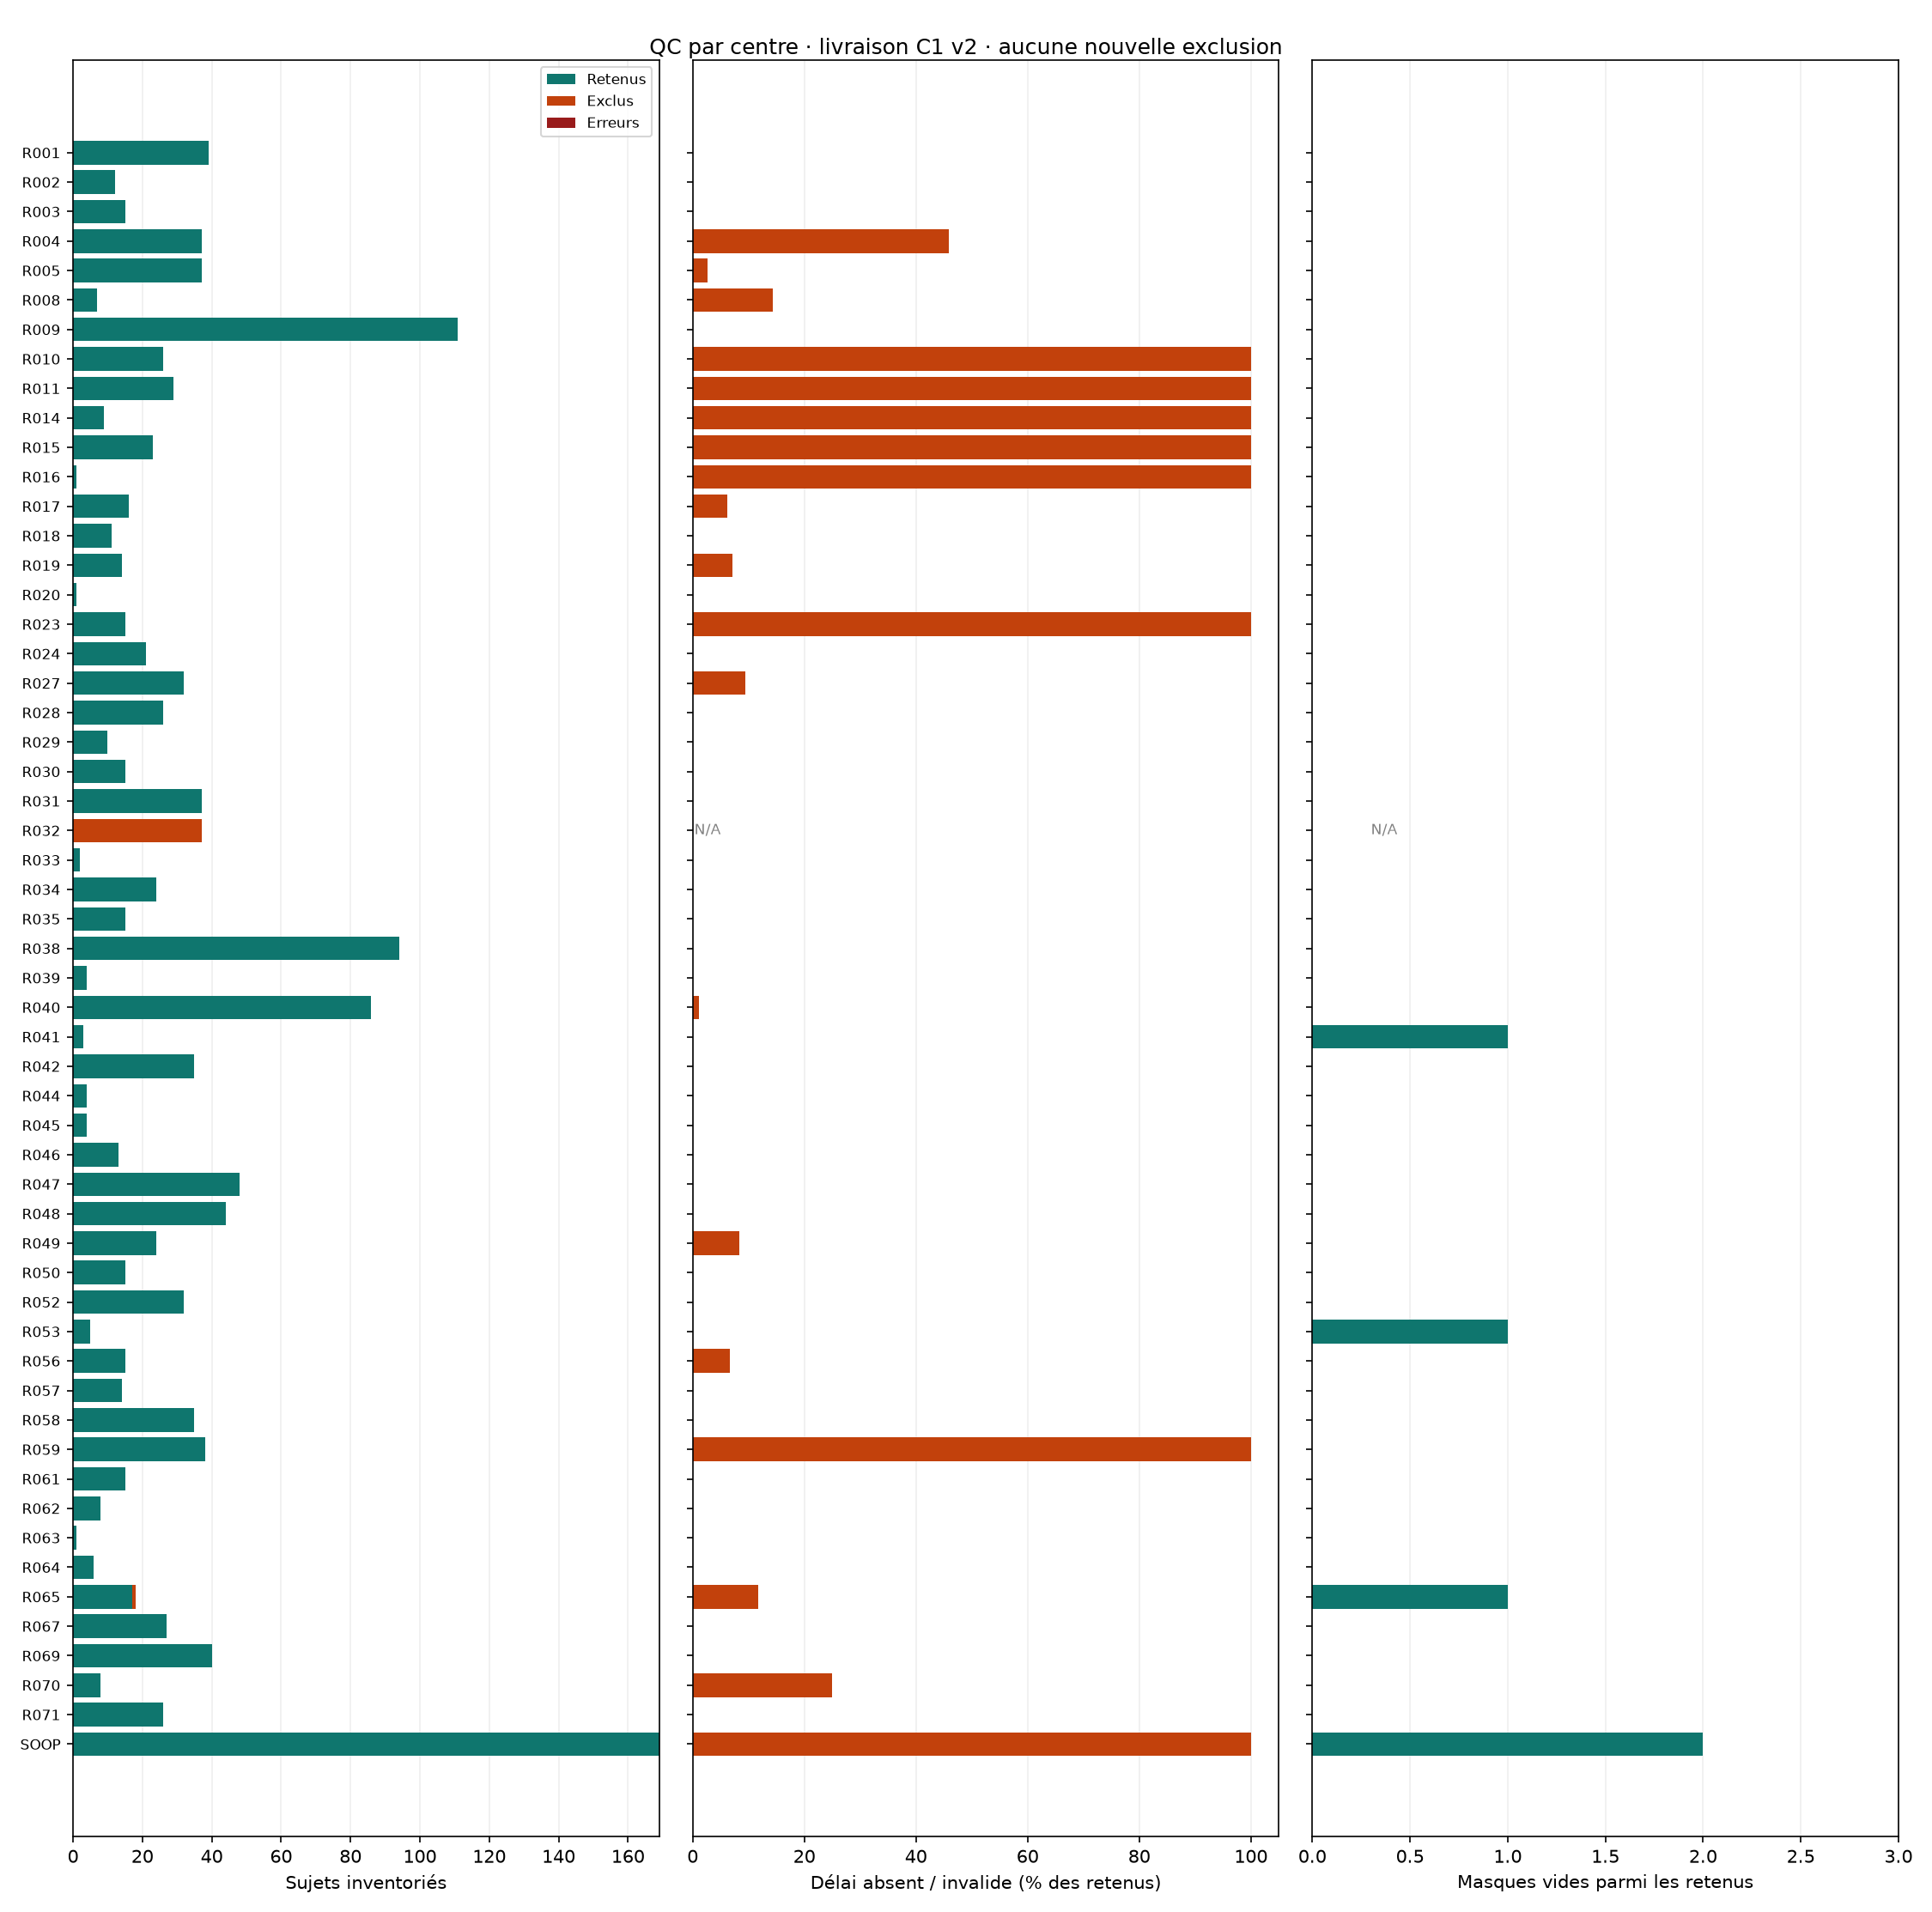
\includegraphics[width=\textwidth]{qc_by_center.png}
  \caption{Synthèse du contrôle qualité par centre : effectifs, exclusions et
  métadonnées manquantes.}
  \label{fig:qc}
\end{figure}

\section{Pipeline de prétraitement Spark}

Chaque sujet est une unité de travail indépendante, traitée en parallèle par
Spark (Python 3.12, Java 17) :

\begin{enumerate}
  \item contrôle des dimensions, des grilles image/masque, de l'affine, des
        valeurs finies et binaires ;
  \item réorientation en RAS et rééchantillonnage à 1 mm isotrope
        (interpolation linéaire pour l'image, plus proche voisin pour les
        masques) ;
  \item normalisation z-score calculée dans le seul masque cérébral, fond
        mis à zéro ;
  \item recadrage autour du cerveau avec une marge de 5 voxels ;
  \item stockage en \fichier{int16} avec un pas de 0,001, soit une erreur
        d'au plus 0,0005 écart-type et deux fois moins d'espace qu'en
        \fichier{float32} ;
  \item signature des entrées et des paramètres pour la reprise, et rapport
        QC pour chaque paire.
\end{enumerate}

Le z-score contraint la moyenne et la variance de chaque scan :
\begin{equation}
  z(v) = \frac{I(v) - \mu_{\text{cerveau}}}{\sigma_{\text{cerveau}}},
  \qquad v \in \text{cerveau}.
\end{equation}
Une correction de biais N4 (ANTsPy) existe en option. Elle n'est pas appliquée
au jeu de référence et aucun bénéfice n'en est revendiqué.

\section{Partitions sans fuite}

Le fichier commun \fichier{splits.json} (version 2) sépare les patients par
centre (tableau~\ref{tab:splits}). Les cinq plis séparent les centres
d'entraînement et de validation ; le test ID de chaque pli ne contient que des
centres présents dans son entraînement.

\begin{table}[H]
  \centering
  \caption{Partition v2 des 1\,415 cas.}
  \label{tab:splits}
  \begin{tabularx}{\textwidth}{lrX}
    \toprule
    \textbf{Partition} & \textbf{Cas} & \textbf{Contenu} \\
    \midrule
    Entraînement / validation & 916 & 5 plis, centres de validation distincts \\
    Test ID                   & 231 & Nouveaux patients des centres vus \\
    Test OOD                  & 268 & 6 centres retirés : R008, R028, R031, R034, R053, SOOP \\
    \midrule
    \textbf{Total}            & \textbf{1\,415} & \\
    \bottomrule
  \end{tabularx}
\end{table}

Les centres OOD ont été choisis en variant leur taille et leur distance
d'intensité ; un écart de distance ID/OOD n'est donc pas une découverte
indépendante. Aucun hyperparamètre n'est choisi sur le test OOD. L'export au
format nnU-Net contient 916 images d'entraînement, 499 images de test et les
cinq plis. Le split v1 est archivé : v2 retire uniquement le cas R065, sans
déplacer d'autre sujet ni de centre.

\section{Performance du pipeline}

Un pilote sur 8 volumes de centres distincts (un essai par configuration)
mesure le temps de calcul selon le nombre de workers
(tableau~\ref{tab:bench}).

\begin{table}[H]
  \centering
  \caption{Temps de calcul du pipeline sur 8 volumes.}
  \label{tab:bench}
  \begin{tabular}{rrr}
    \toprule
    \textbf{Workers} & \textbf{Temps (s)} & \textbf{Accélération} \\
    \midrule
    1 & 56,59 & $\times$1,00 \\
    2 & 41,46 & $\times$1,36 \\
    4 & 27,63 & $\times$2,05 \\
    8 & 42,54 & $\times$1,33 \\
    \bottomrule
  \end{tabular}
\end{table}

L'accélération maximale est obtenue avec 4 workers. La dégradation à 8 workers
est compatible avec des coûts de concurrence et de ressources ; ce pilote ne
permet pas d'en isoler la cause et n'est pas extrapolé au jeu complet.

% =====================================================================
\chapter{Méthodologie}
\label{chap:methodo}
% =====================================================================

\section{Vue d'ensemble}

Le projet relie plusieurs blocs par des contrats de données
(figure~\ref{fig:pipeline}). Le pipeline produit une seule source de données
(C1) ; tous les autres blocs la lisent, et les modèles renvoient leurs Dice
par cas (C3) aux analyses.

\begin{figure}[H]
  \centering
  \resizebox{\textwidth}{!}{%
  \begin{tikzpicture}[
      box/.style={draw=gray!70, rounded corners=4pt, align=center,
                  minimum width=4.2cm, minimum height=1.6cm, font=\small},
      main/.style={box, draw=accent, fill=accent!10, line width=1pt},
      arr/.style={-{Stealth[length=2.5mm]}, gray!70, thick},
      lbl/.style={font=\scriptsize, text=gray!60!black, align=center}]
    % Ligne 1
    \node[box] (raw) {\textbf{Données brutes ATLAS v3}\\1\,453 IRM T1, 55 centres\\masques manuels};
    \node[box, right=1.5cm of raw] (spark) {\textbf{Pipeline Spark}\\QC, RAS, 1 mm, z-score\\Yosra};
    \node[main, right=1.5cm of spark] (c1) {\textbf{Données C1 + splits v2}\\1\,415 cas, 5 plis\\train 916, ID 231, OOD 268};
    % Ligne 2
    \node[box, below=2cm of raw] (gen) {\textbf{Généralisation (C5)}\\intensité, BigAug, FDA, style\\DANN, TENT -- Fayfa};
    \node[box, below=2cm of spark] (models) {\textbf{Modèles de segmentation}\\U-Net 2.5D, ML, nnU-Net\\Anas, Fayfa};
    \node[box, below=2cm of c1] (an) {\textbf{Analyses S5--S10}\\distances, empreinte, S7, S8\\Yosra};
    % Ligne 3
    \node[box, below=1.8cm of models, minimum width=6cm] (demo) {\textbf{Démo et frontend web}\\FastAPI, Gradio, NiiVue, atlas\\Yosra};
    % Flèches
    \draw[arr] (raw) -- (spark);
    \draw[arr] (spark) -- (c1);
    \draw[gray!70, thick] (c1.south) -- ++(0,-0.9) coordinate (bus);
    \draw[arr] (bus) -| (gen.north);
    \draw[arr] (bus) -| (models.north);
    \draw[arr] (bus) -- (an.north);
    \node[lbl, above] at ($(bus)!0.5!(bus -| gen.north)$) {chargées par pli};
    \draw[arr] (gen) -- node[lbl, above=2pt] {transfor-\\mations} (models);
    \draw[arr] (models) -- node[lbl, above=2pt] {Dice par\\cas (C3)} (an);
    \draw[arr] (models) -- node[lbl, right] {prédiction} (demo);
    \draw[arr] (an.south) |- node[lbl, pos=0.25, right] {figures et rapports} (demo.east);
  \end{tikzpicture}}
  \caption{Vue d'ensemble du projet et des contrats de données.}
  \label{fig:pipeline}
\end{figure}

\section{Baselines de segmentation}

\subsection{Réseau convolutif}

Le modèle principal est un U-Net à encodeur ResNet-34 pré-entraîné sur
ImageNet (24,4 M paramètres). Il reçoit une entrée 2.5D : trois coupes
axiales voisines $(z-1, z, z+1)$ empilées comme les trois canaux d'une image
couleur, de taille $224 \times 192$. Ce choix réutilise les poids ImageNet et
tient dans les 4 Go du GPU disponible (RTX 2050). Le tableau~\ref{tab:cnn}
résume la configuration.

\begin{table}[H]
  \centering
  \caption{Configuration d'entraînement du CNN.}
  \label{tab:cnn}
  \begin{tabularx}{\textwidth}{lX}
    \toprule
    \textbf{Paramètre} & \textbf{Valeur} \\
    \midrule
    Architecture    & U-Net, encodeur ResNet-34 (ImageNet), sortie sigmoïde \\
    Perte           & Entropie croisée binaire + Dice souple \\
    Optimiseur      & AdamW, taux $5 \times 10^{-4}$, décroissance $10^{-4}$ \\
    Planification   & Décroissance polynomiale $(1 - t/T)^{0,9}$ \\
    Budget          & 8 minutes par variante (2\,600 à 4\,500 itérations), identique pour toutes \\
    Lot             & 16 coupes, précision mixte \\
    Échantillonnage & 60\,\% de coupes avec lésion, 40\,\% aléatoires \\
    Augmentation    & Miroir gauche--droite, échelle 0,85--1,15 et décalage $\pm$0,15 d'intensité, bruit gaussien \\
    Inférence       & Toutes les coupes et leur miroir moyennés (TTA), seuil 0,5 \\
    \bottomrule
  \end{tabularx}
\end{table}

La perte combine deux termes, où $p$ est la probabilité prédite et $g$ la
vérité terrain :
\begin{equation}
  \mathcal{L} = \mathcal{L}_{\text{BCE}}(p, g)
  + \left(1 - \frac{2\sum_v p_v g_v}{\sum_v p_v + \sum_v g_v}\right).
\end{equation}

Quatre variantes mesurent l'apport du transfert : fine-tuning complet, début
de l'encodeur gelé (conv1, layer1, layer2), encodeur entier gelé (seul le
décodeur apprend, 3,2 M poids), et initialisation aléatoire comme contrôle.

\subsection{Modèles classiques}

Trois modèles (régression logistique, forêt aléatoire, gradient boosting)
classent chaque voxel à partir de 11 caractéristiques : intensité et versions
lissées ($\sigma$ = 1, 2, 4 mm), texture locale, asymétrie gauche--droite et
position dans le cerveau. L'asymétrie est la plus importante (28\,\% de
l'importance de la forêt), car un AVC touche un seul hémisphère. Les seuils
de décision sont choisis sur 15 autres patients d'entraînement.

\subsection{nnU-Net}

Un nnU-Net 3D complet est préparé, avec l'export au format attendu et les
cinq plis. Il demande un GPU plus puissant que celui du poste utilisé.

\section{Généralisation inter-centres (contrat C5)}

Une bibliothèque de transformations, appliquées uniquement à l'entraînement,
simule la variabilité des centres. Chaque famille dispose de sa
configuration YAML :
\begin{itemize}
  \item augmentation d'intensité (gamma 0,68--1,79, contraste 0,77--1,53) ;
  \item BigAug ;
  \item randomisation du style (GIN, RandConv) ;
  \item méthode de Fourier FDA ;
  \item harmonisation par appariement d'histogramme (référence R059 ou R071
        selon le pli).
\end{itemize}
Le calibrage utilise uniquement les 916 sujets d'entraînement du split v2. Un
test échoue si un centre de test sert à un réglage.

\section{Adaptation de domaine}

\subsection{DANN}

DANN ajoute au U-Net un classifieur de centre branché sur le bottleneck, via
une couche d'inversion de gradient. Le classifieur apprend à reconnaître le
centre ; l'encodeur reçoit le gradient opposé, multiplié par $-\lambda$, et
apprend à effacer l'empreinte du centre. Le coefficient suit la
planification de Ganin, avec $p$ l'avancement de l'entraînement :
\begin{equation}
  \lambda(p) = \frac{2}{1 + \exp(-10\,p)} - 1, \qquad p \in [0, 1].
\end{equation}
La perte totale est $\mathcal{L}_{\text{Dice+CE}} + w \cdot
\mathcal{L}_{\text{CE centre}}$ avec $w = 1$. Seuls les centres
d'entraînement du pli sont utilisés par le classifieur.

\subsection{TENT}

TENT adapte un modèle déjà entraîné sur un nouveau centre, sans étiquettes.
Seuls les paramètres affines ($\gamma$, $\beta$) des couches de normalisation
apprennent, en minimisant l'entropie moyenne des prédictions dans le cerveau :
\begin{equation}
  \mathcal{H} = -\frac{1}{|B|}\sum_{v \in B}
  \big[p_v \log p_v + (1-p_v)\log(1-p_v)\big],
\end{equation}
où $B$ est le masque cérébral ; le fond, prédit avec certitude, écraserait
sinon la moyenne. La fonction \fichier{reset()} restaure exactement l'état
d'origine entre deux centres. TENT exige des normalisations affines : le
U-Net MONAI par défaut n'en possède pas.

Ces deux modules sont testés sur de petits U-Net 3D et sur de vrais patches
C1. Ce ne sont pas encore des poids entraînés.

\section{Mesure du décalage et analyses}

\begin{description}
  \item[S5 -- Distances.] Wasserstein et MMD entre chaque centre et la
        référence, avant et après prétraitement.
  \item[S6 -- Empreinte du centre.] Capacité à deviner le centre depuis
        l'histogramme d'intensité : cinq plis stratifiés, exactitude
        équilibrée, contrôle à labels mélangés.
  \item[S7 -- Prédiction d'échec.] Relation entre la distance au train du
        pli et l'erreur $1 - \text{Dice}$ par centre, en validation
        \emph{leave-one-center-out}.
  \item[S8 -- Délai post-AVC.] Modèles linéaires emboîtés (constante,
        centre, $\log(1 + \text{jours})$, centre + temps) et permutations
        intra-centre (999, graine 2026).
  \item[S9--S10 -- Représentations.] Empreinte du centre dans les
        caractéristiques du réseau (baseline, augmentation, DANN), protocole
        préparé.
\end{description}

\section{Métriques}

La métrique principale est le coefficient de Dice entre la prédiction $P$ et
la vérité terrain $G$ :
\begin{equation}
  \text{Dice}(P, G) = \frac{2\,|P \cap G|}{|P| + |G|}.
\end{equation}
La distance de Hausdorff au 95\textsuperscript{e} percentile (HD95), l'erreur
absolue de volume et le F1 par lésion la complètent. L'écart de
généralisation est défini par $\text{Dice}_{\text{ID}} -
\text{Dice}_{\text{OOD}}$.

% =====================================================================
\chapter{Résultats et analyses}
\label{chap:resultats}
% =====================================================================

\section{Segmentation : baselines}

Ces résultats proviennent d'un protocole historique (903 cas
d'entraînement, 226 de validation ID, 287 OOD issus de 14 centres). Ils ne
sont pas les résultats des cinq plis du split v2. Tous les modèles sont
évalués sur les mêmes 300 patients (tableau~\ref{tab:baselines},
figure~\ref{fig:dice}).

\begin{table}[H]
  \centering
  \caption{Dice moyen des baselines sur les mêmes 300 patients de test.}
  \label{tab:baselines}
  \begin{tabular}{lcc}
    \toprule
    \textbf{Modèle} & \textbf{ID} & \textbf{OOD} \\
    \midrule
    CNN pré-entraîné, fine-tuning complet     & \textbf{0,50} & \textbf{0,52} \\
    CNN pré-entraîné, début d'encodeur gelé   & 0,49 & 0,52 \\
    CNN pré-entraîné, encodeur entier gelé    & 0,47 & 0,51 \\
    CNN sans pré-entraînement                 & 0,40 & 0,44 \\
    \midrule
    Gradient boosting                         & 0,33 & 0,38 \\
    Forêt aléatoire                           & 0,28 & 0,33 \\
    Régression logistique                     & 0,16 & 0,21 \\
    \bottomrule
  \end{tabular}
\end{table}

\begin{figure}[H]
  \centering
  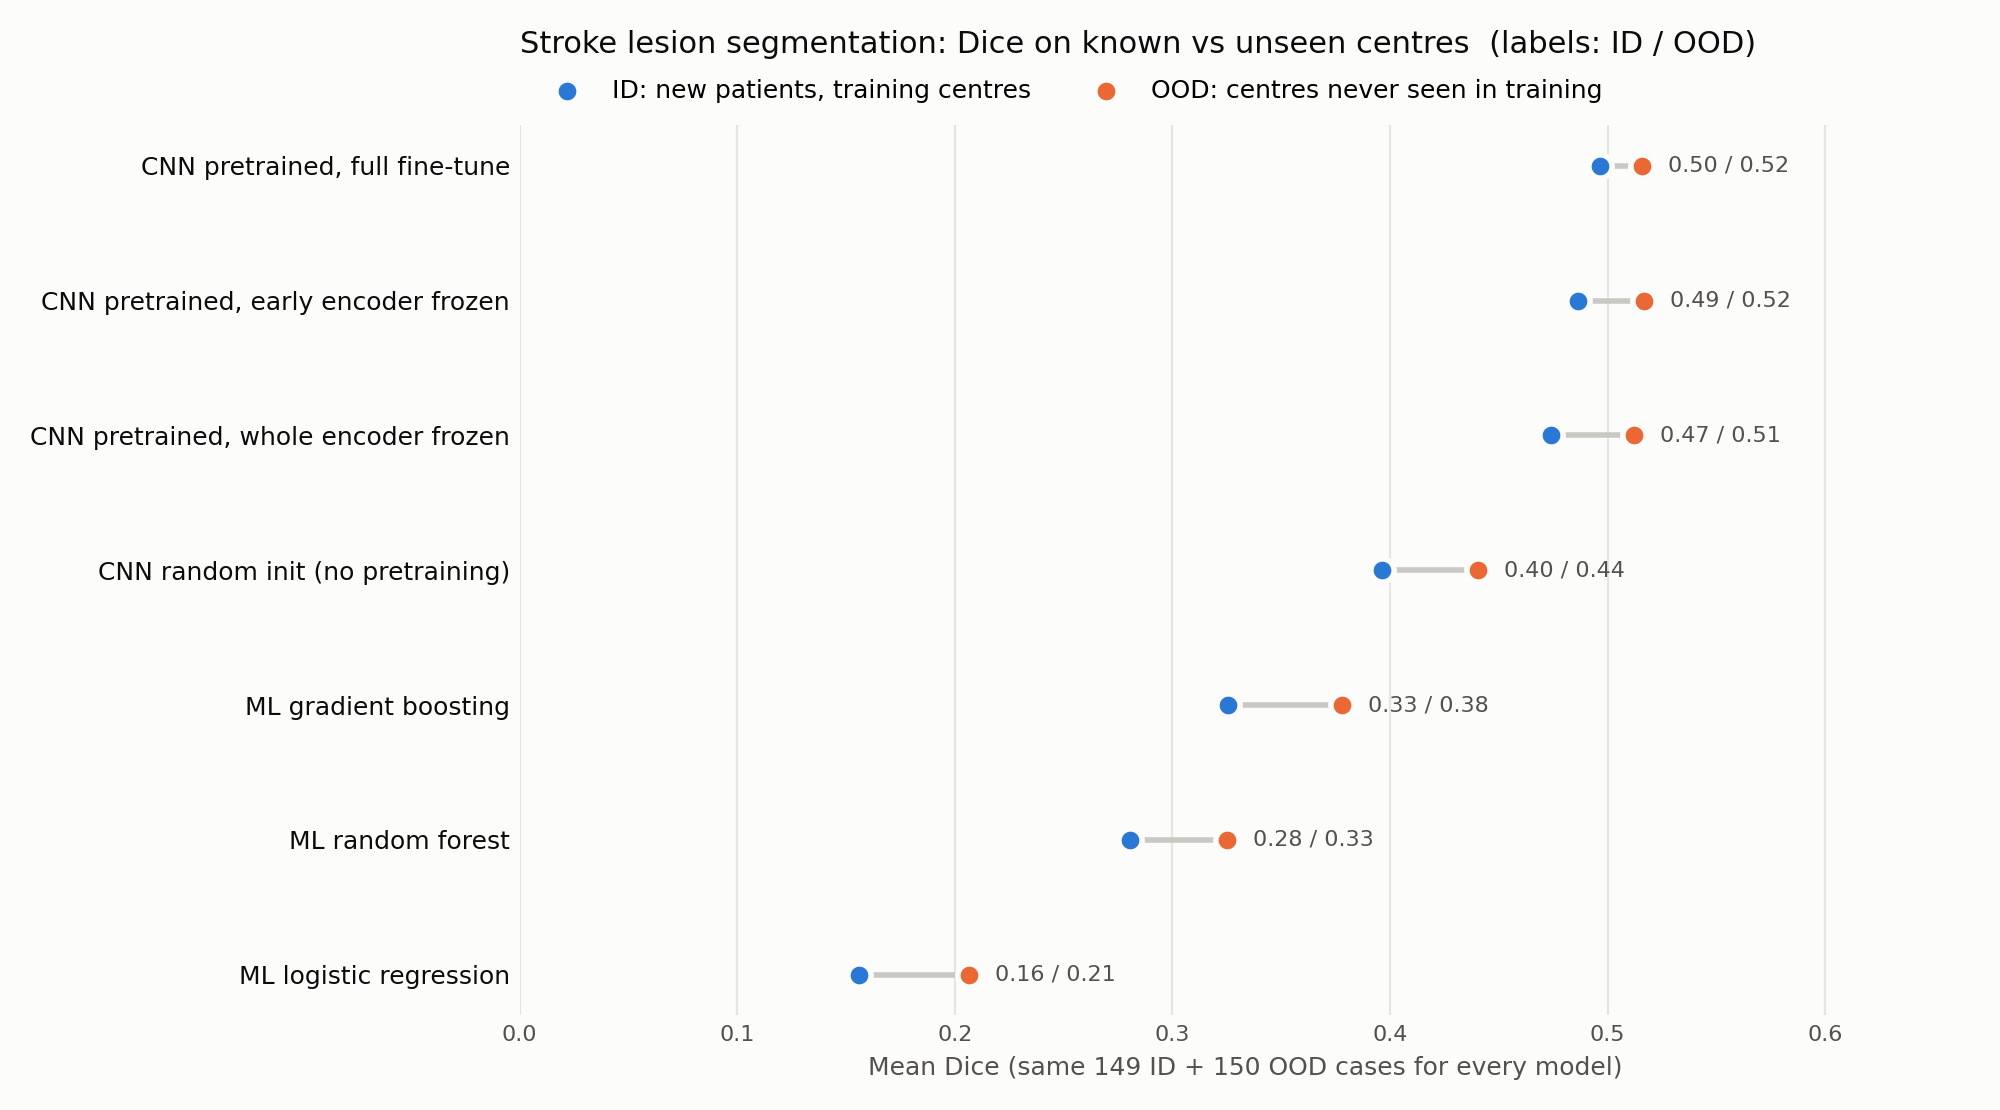
\includegraphics[width=0.85\textwidth]{fig1_dice_id_vs_ood.png}
  \caption{Dice ID et OOD des baselines.}
  \label{fig:dice}
\end{figure}

Sur les 512 patients de test, le meilleur CNN atteint un Dice de 0,47 en ID
et 0,53 en OOD. Quatre constats ressortent :
\begin{itemize}
  \item le pré-entraînement ImageNet apporte environ +0,10 de Dice (0,50
        contre 0,40 en ID) ;
  \item les CNN dépassent nettement les modèles classiques ;
  \item le Dice dépend surtout de la taille de la lésion
        (figure~\ref{fig:taille}) : en OOD, 0,20 sous 1 mL, 0,44 entre 1 et
        10 mL, 0,70 entre 10 et 50 mL et 0,84 au-delà ;
  \item les lésions OOD sont plus grandes (médiane 5,6 mL contre 3,7 mL), ce
        qui explique leur légère avance : aucune baisse n'est mesurable sur
        les centres inconnus dans ce split.
\end{itemize}
Le meilleur modèle a été choisi sur la validation ID uniquement, jamais sur
le test OOD.

\begin{figure}[H]
  \centering
  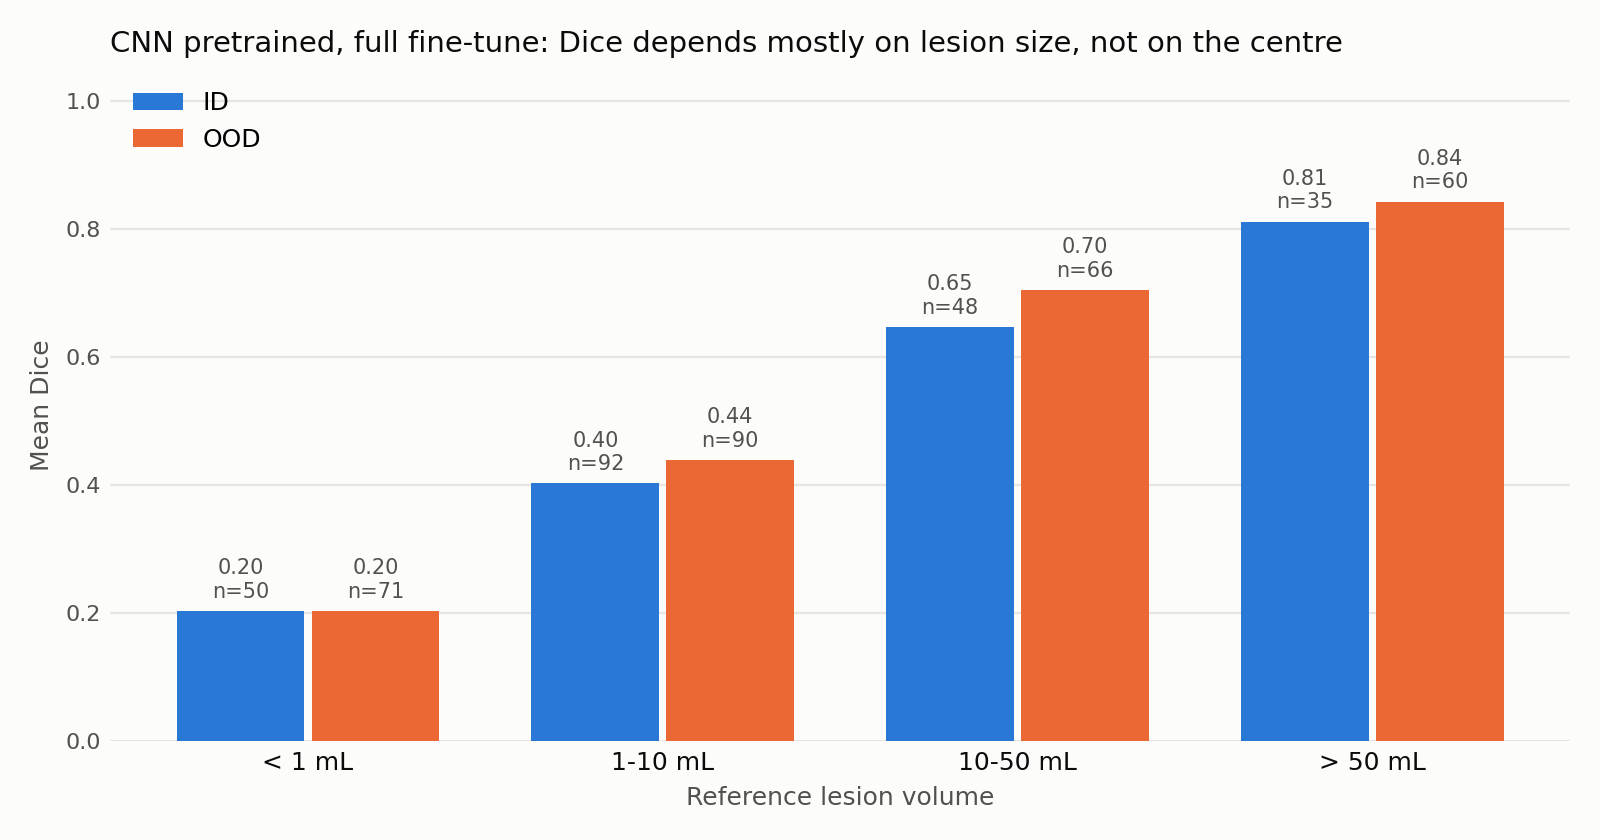
\includegraphics[width=0.75\textwidth]{fig2_dice_by_lesion_size.png}
  \caption{Dice selon la taille de la lésion.}
  \label{fig:taille}
\end{figure}

\begin{figure}[H]
  \centering
  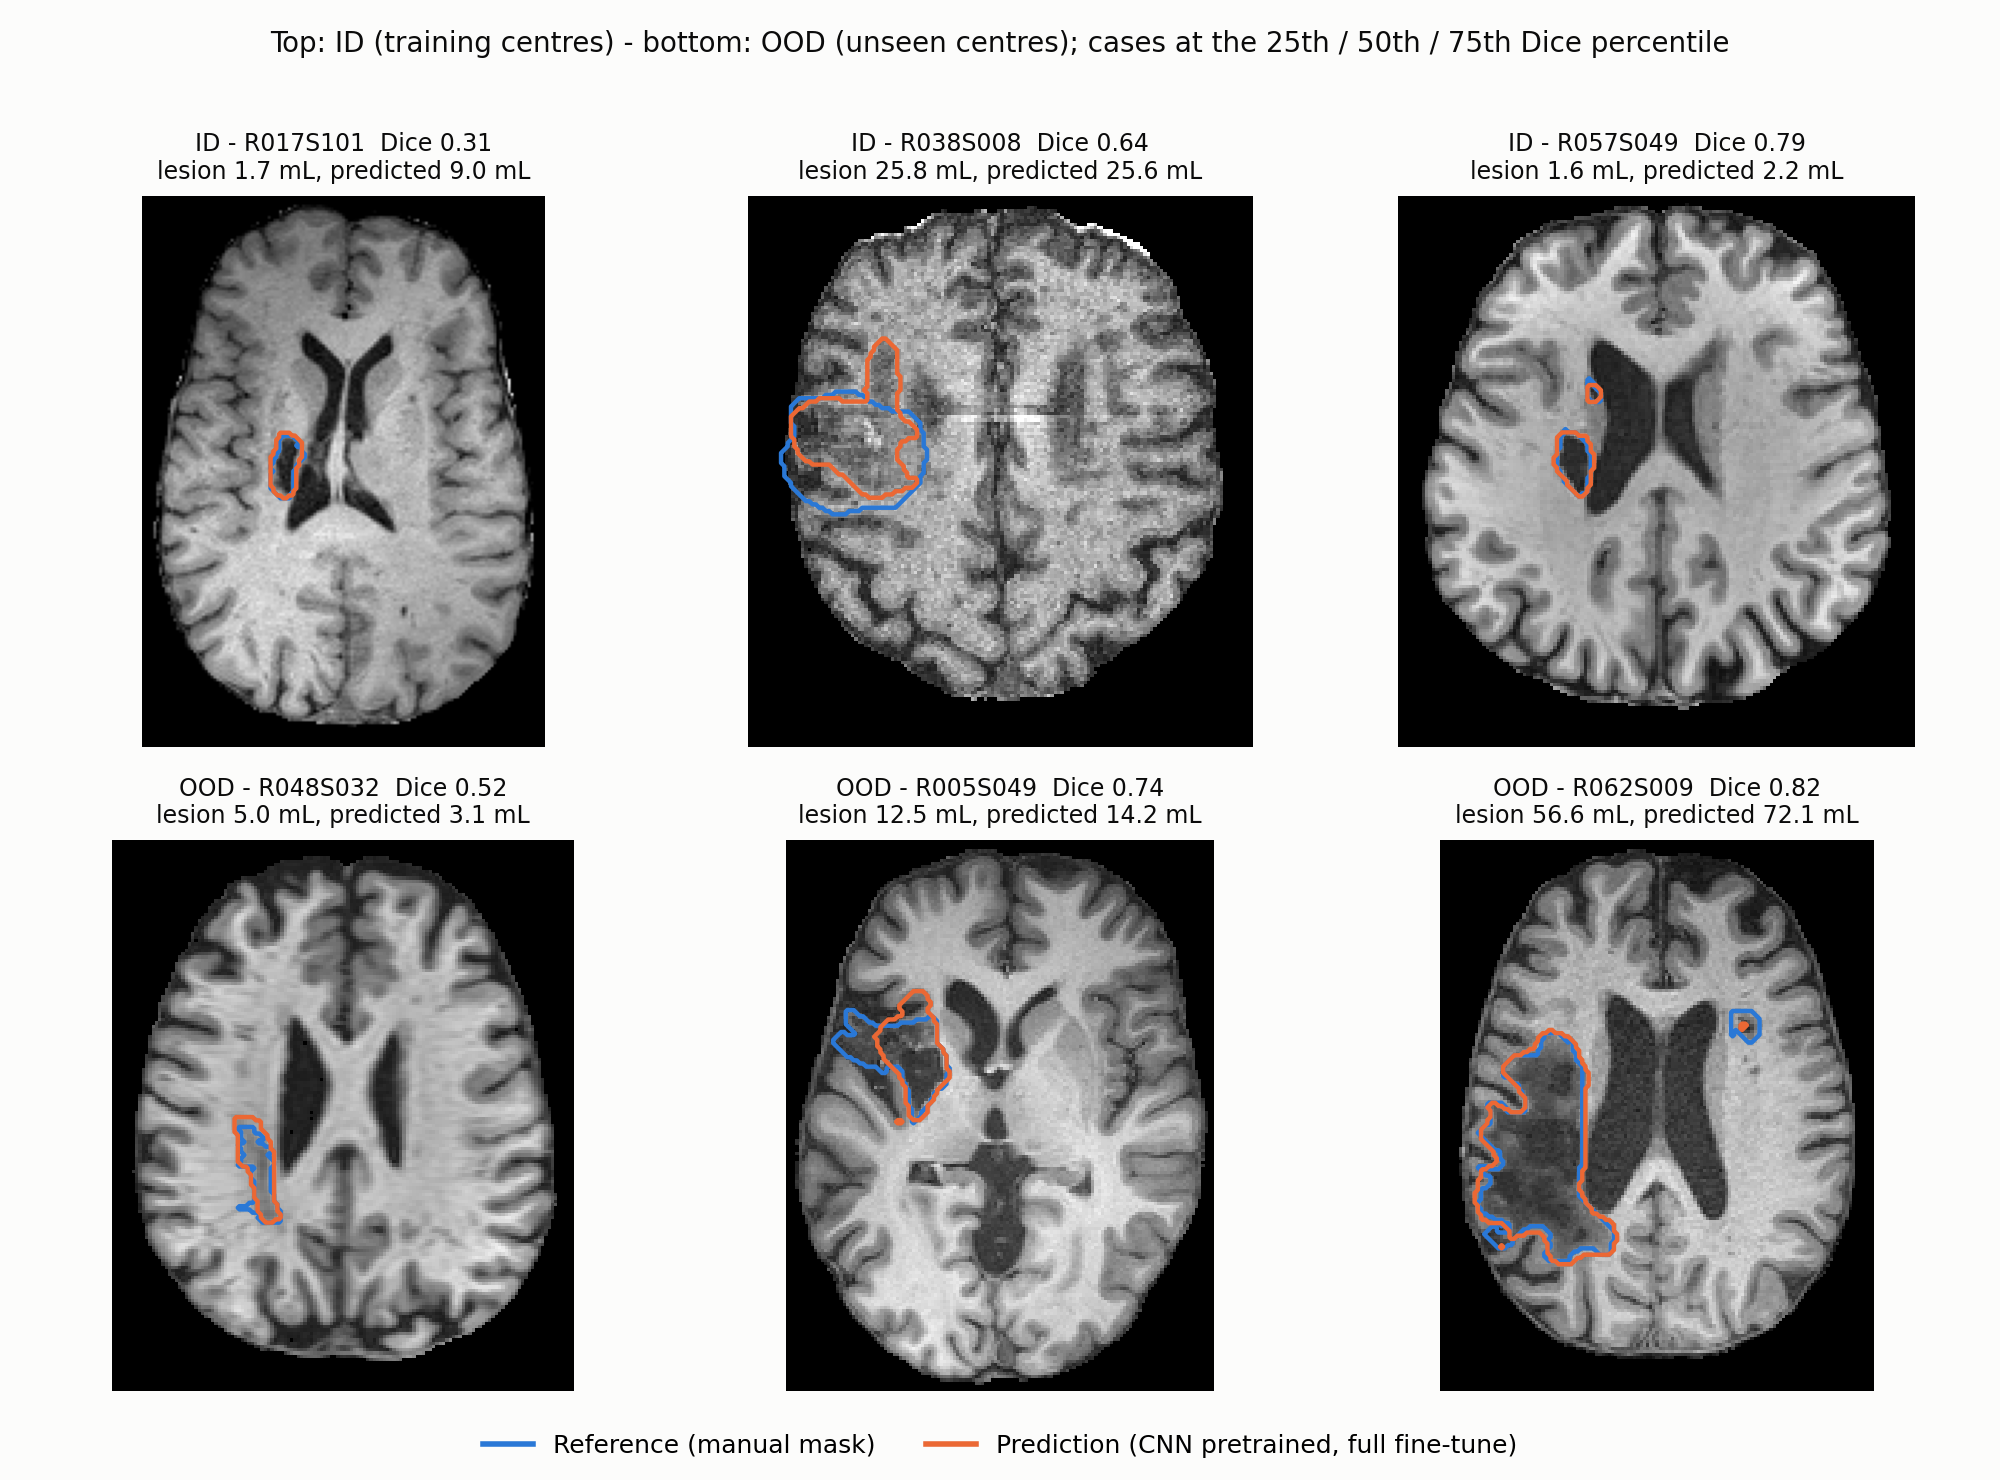
\includegraphics[width=\textwidth]{fig3_examples.png}
  \caption{Exemples de segmentation aux 25\textsuperscript{e},
  50\textsuperscript{e} et 75\textsuperscript{e} percentiles du Dice. En
  haut : ID ; en bas : OOD. Bleu : masque manuel ; orange : prédiction du
  meilleur CNN.}
  \label{fig:exemples}
\end{figure}

\section{Décalage entre centres (S5)}

Sur 1\,415 sujets de 54 centres, la distance relative médiane au centre de
référence passe de 0,1315 avant prétraitement à 0,0376 après. Wasserstein et
MMD sont fortement corrélées (0,842 pour les centres d'au moins cinq scans).
La médiane de Wasserstein vaut 0,0376 en ID et 0,0900 en OOD ; cet écart est
en partie dû à la sélection des centres OOD.

La figure~\ref{fig:avantapres} montre l'effet du prétraitement : avant, les
intensités moyennes s'étalent sur plusieurs ordres de grandeur ; après, les
médianes du z-score restent proches de zéro, mais des différences de forme
subsistent entre centres.

\begin{figure}[H]
  \centering
  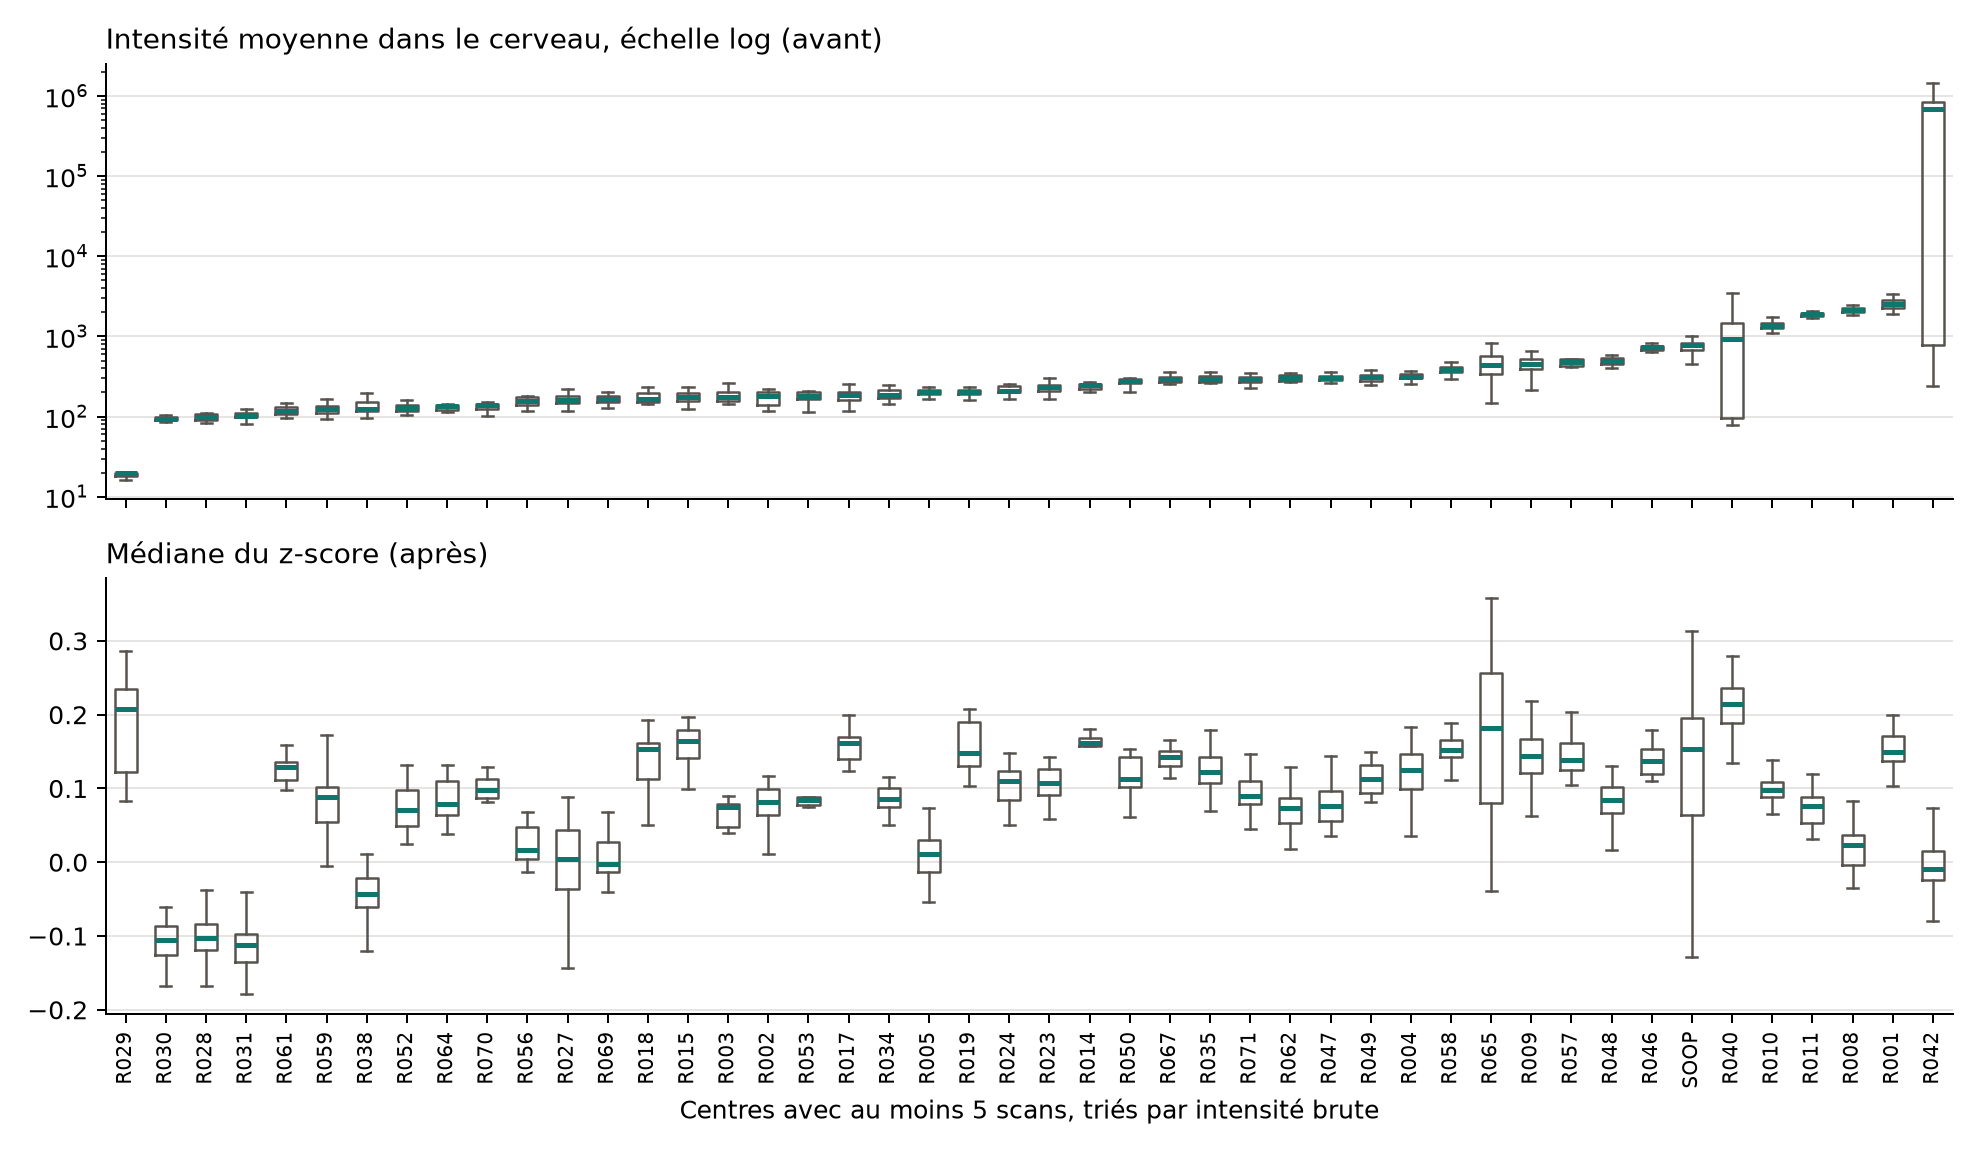
\includegraphics[width=\textwidth]{s5_avant_apres_par_centre.png}
  \caption{Intensité par centre avant (échelle logarithmique) et après
  prétraitement (médiane du z-score).}
  \label{fig:avantapres}
\end{figure}

\begin{figure}[H]
  \centering
  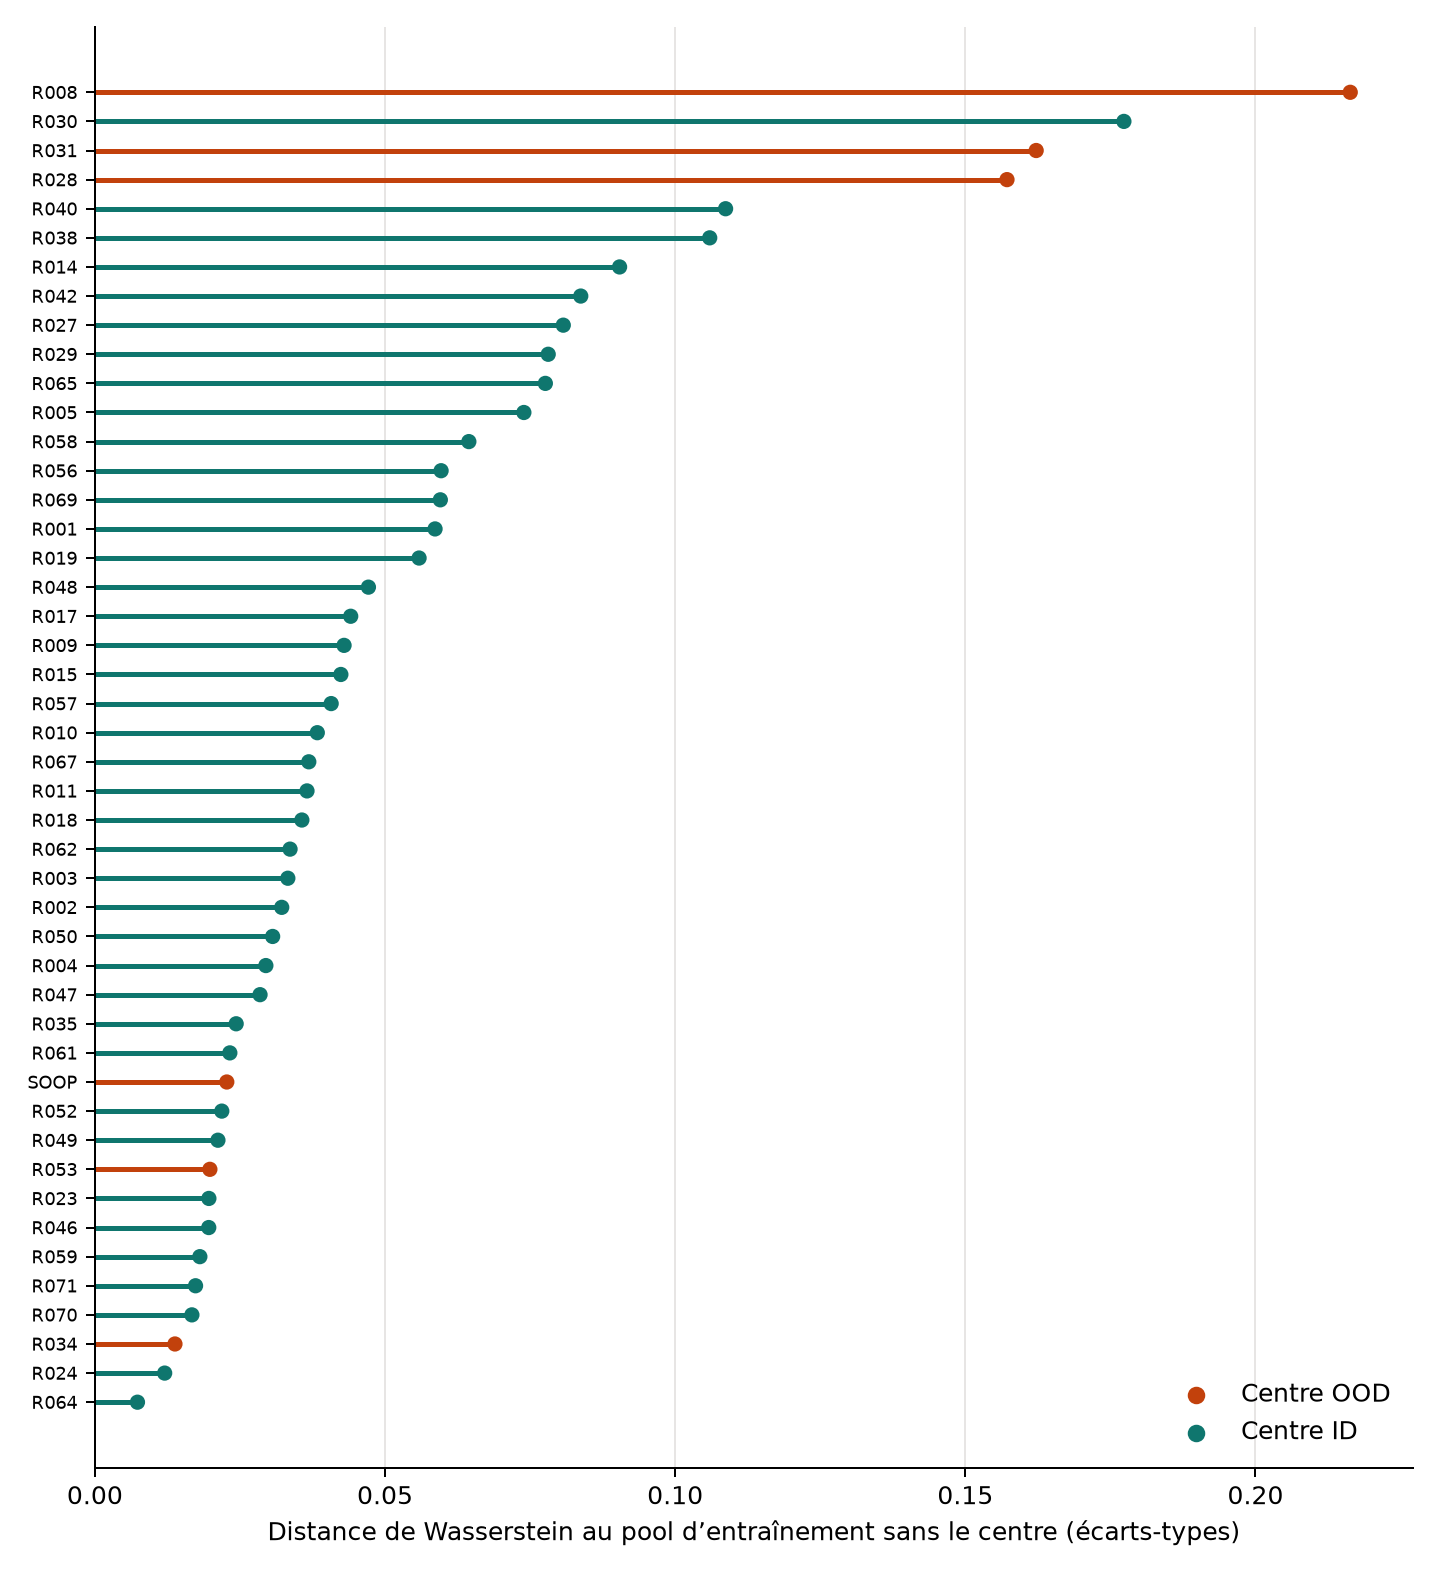
\includegraphics[width=0.9\textwidth]{s5_distances_centres.png}
  \caption{Distances entre chaque centre et la référence.}
  \label{fig:distances}
\end{figure}

\section{Empreinte du centre (S6)}

Le test S6 retient 1\,140 scans de 25 centres. Un classifieur tente de
deviner le centre à partir de l'histogramme d'intensité
(tableau~\ref{tab:empreinte}, figure~\ref{fig:empreinte}).

\begin{table}[H]
  \centering
  \caption{Reconnaissance du centre à partir de l'histogramme d'intensité.}
  \label{tab:empreinte}
  \begin{tabular}{lr}
    \toprule
    \textbf{Représentation} & \textbf{Exactitude équilibrée} \\
    \midrule
    Histogramme avant prétraitement (32 classes) & 69,7\,\% \\
    Histogramme après prétraitement (30 classes) & 48,9\,\% \\
    Contrôle à labels mélangés                   & 4,0\,\% \\
    Hasard (25 centres)                          & 4\,\% \\
    \bottomrule
  \end{tabular}
\end{table}

\begin{figure}[H]
  \centering
  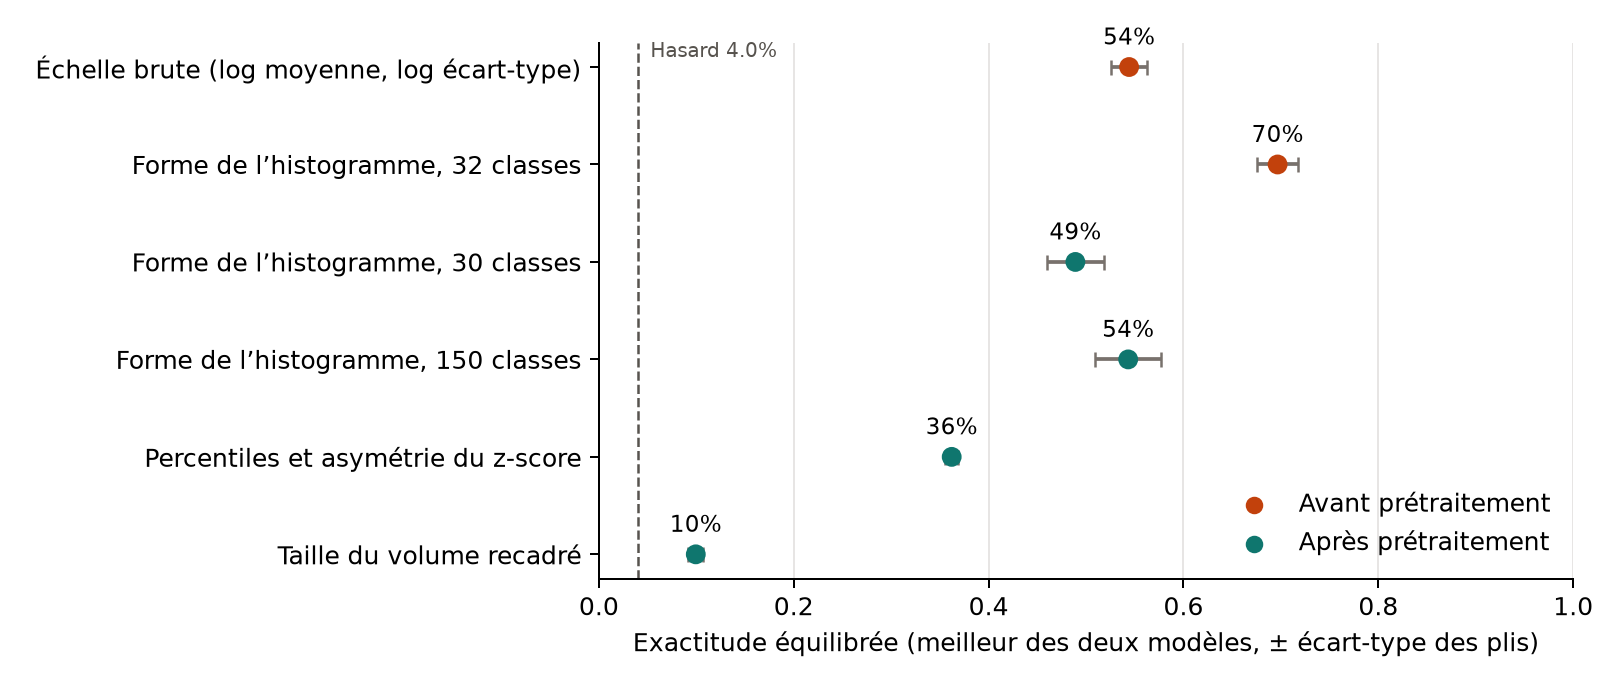
\includegraphics[width=0.8\textwidth]{s6_empreinte_centre.png}
  \caption{Empreinte du centre avant et après prétraitement.}
  \label{fig:empreinte}
\end{figure}

Une évaluation complémentaire (912 sujets d'entraînement, 228 réservés,
10\,000 rééchantillonnages intra-centre) quantifie l'incertitude
(figure~\ref{fig:ic}). Pour la forêt aléatoire, le score passe de 70,1\,\%
[64,6 ; 75,5] à 51,1\,\% [45,3 ; 57,0], soit une différence appariée de
$-19{,}0$ points, IC 95\,\% [$-25{,}5$ ; $-12{,}6$]. Pour la régression
logistique, la différence est de $-21{,}5$ points [$-27{,}4$ ; $-15{,}5$].

\begin{figure}[H]
  \centering
  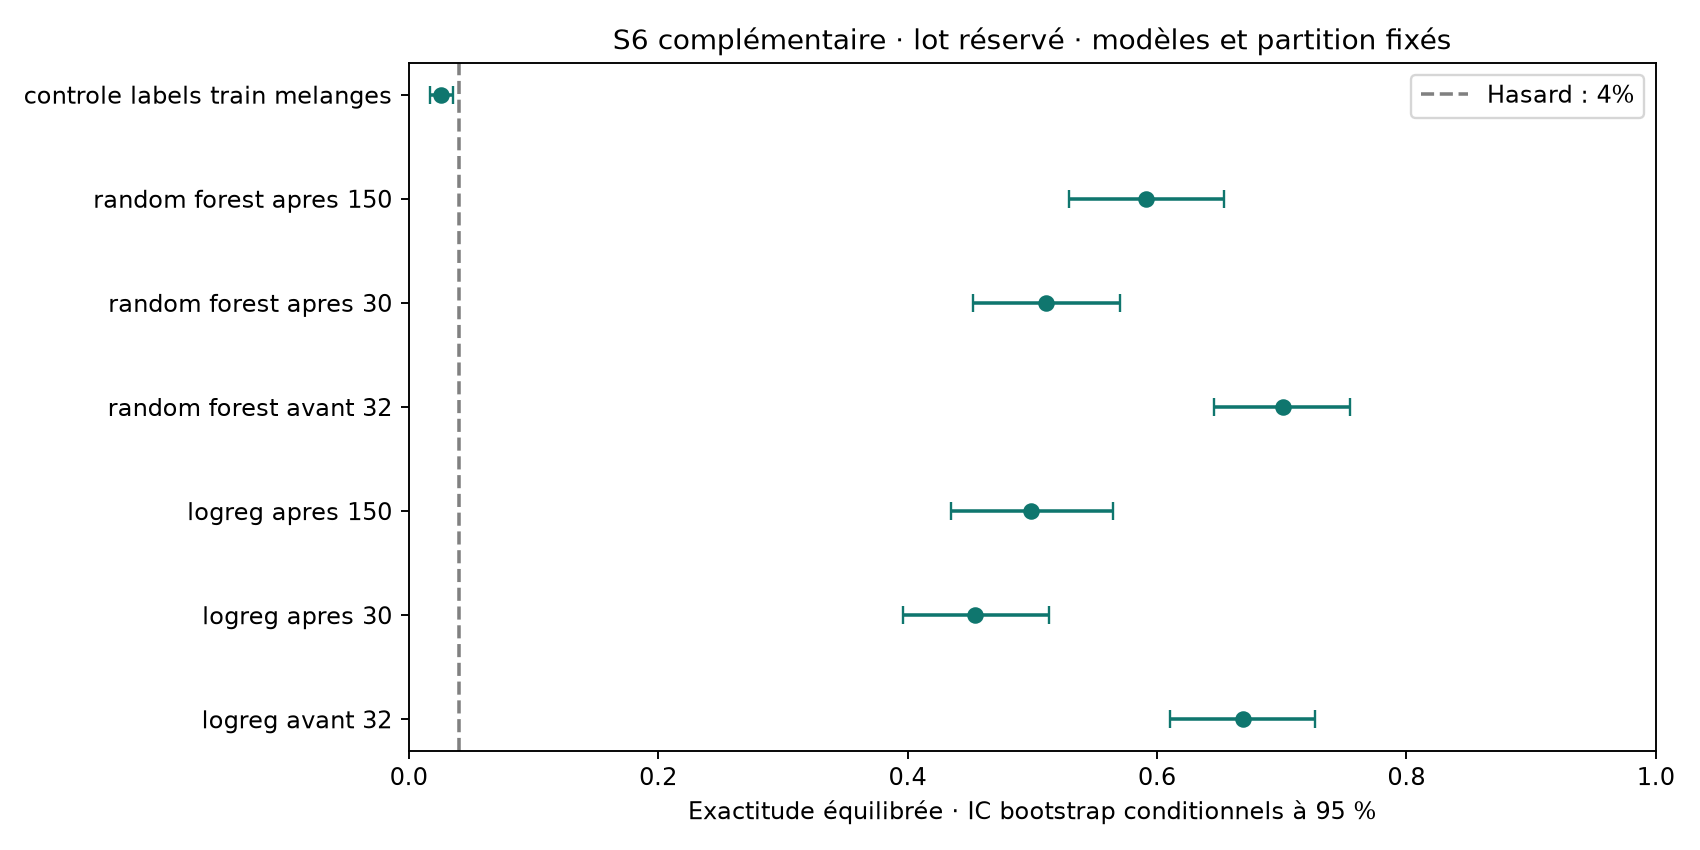
\includegraphics[width=0.8\textwidth]{confidence_intervals.png}
  \caption{Intervalles de confiance à 95\,\% de l'exactitude équilibrée.}
  \label{fig:ic}
\end{figure}

Le prétraitement efface donc une partie de l'empreinte, mais le centre reste
reconnaissable bien au-dessus du hasard. Ces intervalles conditionnent sur
les modèles et la partition fixés, et une empreinte reconnaissable
n'implique pas à elle seule une baisse du Dice.

\section{Délai post-AVC et Dice (S8, exploratoire)}

Le délai post-AVC est disponible pour 1\,073 sujets (médiane 365 jours) ; il
dépend fortement du centre ($\eta^2 = 0{,}7475$, figure~\ref{fig:delai}).
L'analyse doit donc toujours tenir compte du centre.

\begin{figure}[H]
  \centering
  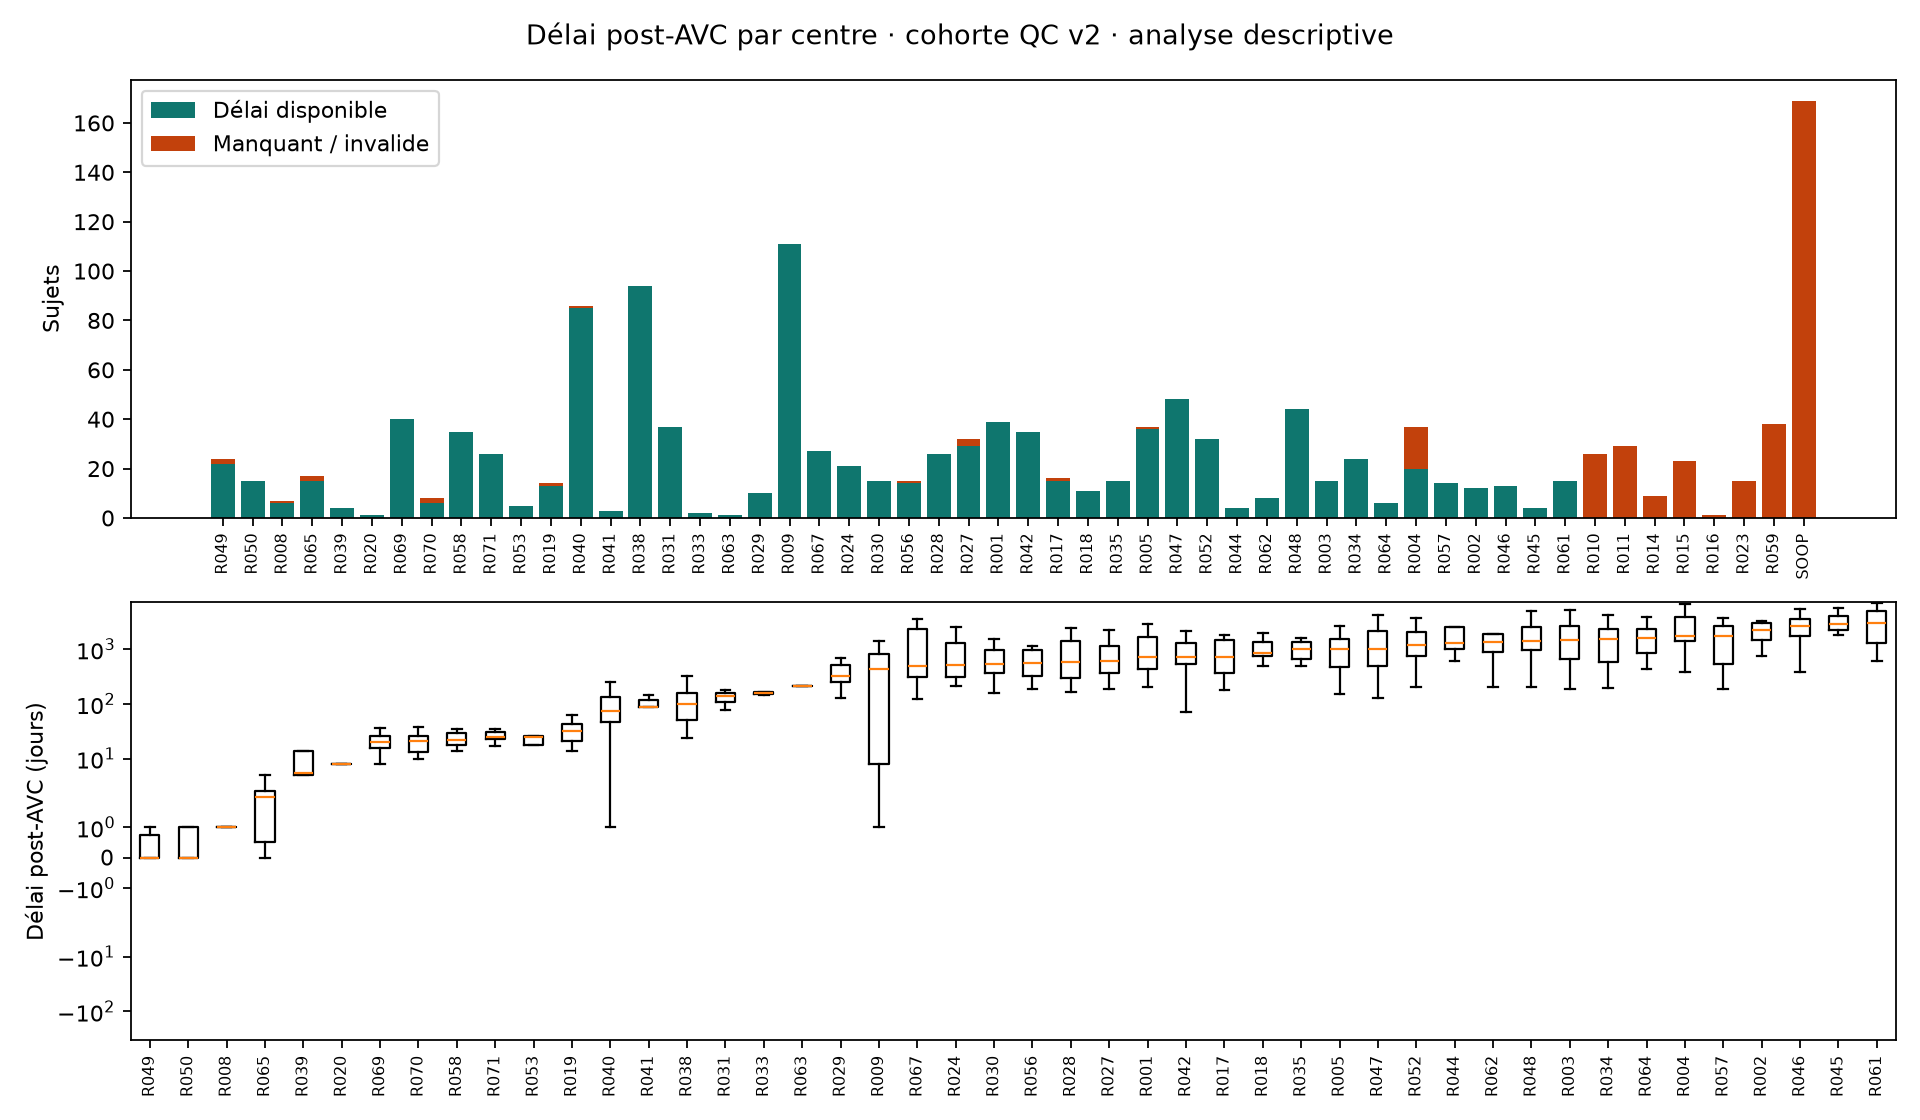
\includegraphics[width=0.85\textwidth]{s8_delai_metadonnees.png}
  \caption{Délai post-AVC et métadonnées par centre.}
  \label{fig:delai}
\end{figure}

Sur les scores historiques du meilleur CNN (167 cas ID de 31 centres, 257 cas
OOD de 12 centres), on ajoute $\log(1 + \text{délai})$ à un modèle déjà
ajusté sur le centre (tableau~\ref{tab:s8}, figure~\ref{fig:tempsdice}).

\begin{table}[H]
  \centering
  \caption{Gain de $R^2$ apporté par le délai post-AVC, à centre fixé.}
  \label{tab:s8}
  \begin{tabular}{lccc}
    \toprule
    \textbf{Groupe} & \textbf{Gain de $R^2$} & \textbf{$p$ (permutations)} & \textbf{Gain avec volume} \\
    \midrule
    ID  & 0,000046 & 0,911 & 0,000711 \\
    OOD & 0,03808  & 0,001 & 0,000217 \\
    \bottomrule
  \end{tabular}
\end{table}

\begin{figure}[H]
  \centering
  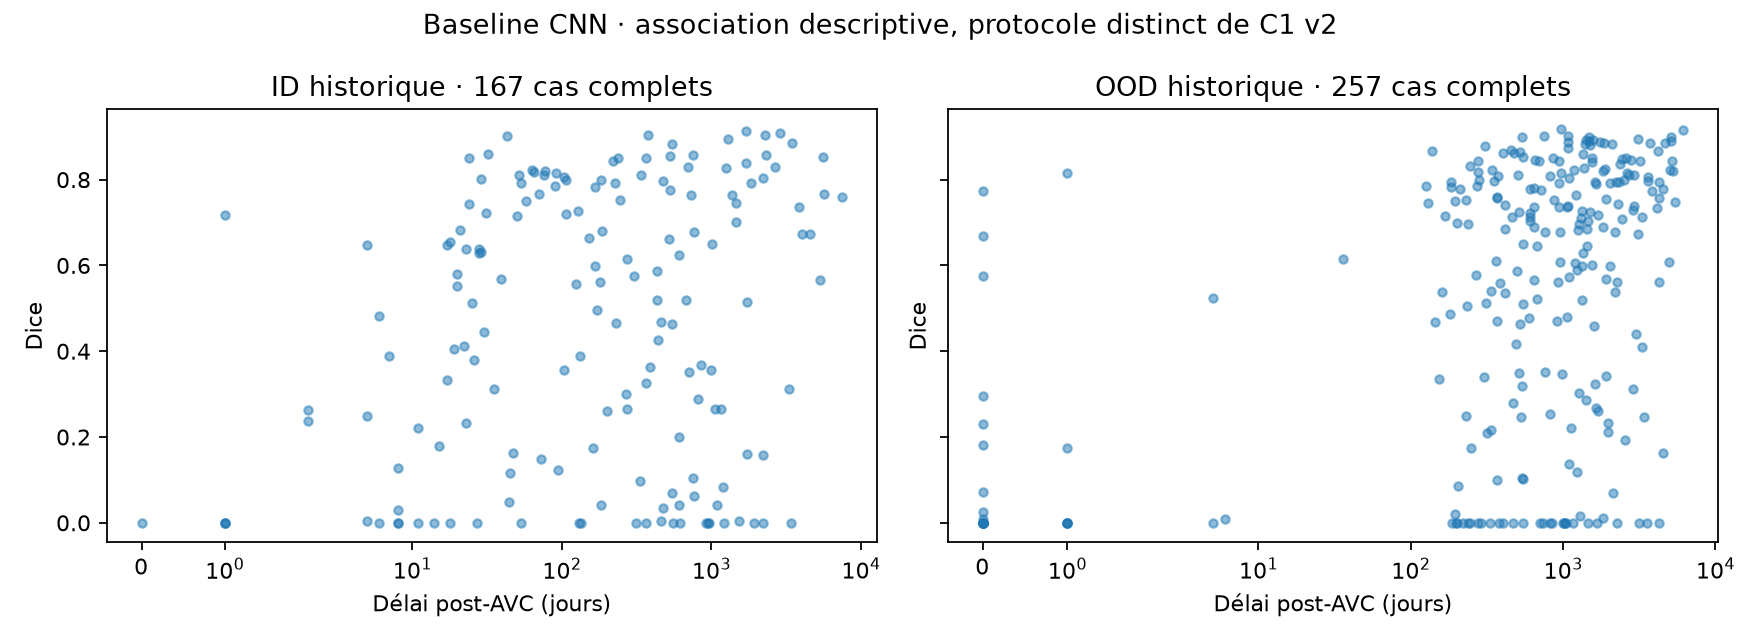
\includegraphics[width=0.8\textwidth]{time_dice.png}
  \caption{Dice en fonction du délai post-AVC (scores historiques).}
  \label{fig:tempsdice}
\end{figure}

L'association OOD disparaît presque une fois le volume lésionnel pris en
compte : elle ne permet pas d'attribuer un effet causal au temps. Ces tests
sont exploratoires, sans correction de multiplicité, et la partition diffère
de C1 v2.

\section{Résultats encore attendus}

Les résultats RQ1--RQ3 sur le split v2 (nnU-Net, Transformers,
augmentation, DANN, TENT), la prédiction d'échec S7 et la comparaison des
représentations S9--S10 attendent les prédictions et les checkpoints de
l'équipe modèles. Les outils sont prêts et testés ; aucun Dice n'est simulé.

% =====================================================================
\chapter{Application et démonstration}
% =====================================================================

Une application web locale présente tout le projet et permet d'analyser une
IRM. Elle affiche les coupes et la vue 3D, calcule le volume lésionnel en mL
et indique toujours s'il s'agit d'un masque fourni ou d'une prédiction.

\section{Architecture}

\begin{figure}[H]
  \centering
  \resizebox{\textwidth}{!}{%
  \begin{tikzpicture}[
      box/.style={draw=gray!70, rounded corners=4pt, align=center,
                  minimum width=4.2cm, minimum height=1.9cm, font=\small},
      main/.style={box, draw=accent, fill=accent!10, line width=1pt},
      arr/.style={-{Stealth[length=2.5mm]}, gray!70, thick},
      lbl/.style={font=\scriptsize, text=gray!60!black}]
    \node[box] (nav) {\textbf{Navigateur}\\HTML, CSS, JS sans build\\graphiques SVG\\NiiVue : coupes et 3D};
    \node[main, right=1.8cm of nav] (api) {\textbf{Serveur FastAPI}\\\fichier{server.py}\\\fichier{/api/overview} \dots\ \fichier{/figures}\\\fichier{POST /api/analyze}};
    \node[box, right=1.8cm of api, yshift=1.3cm, minimum height=1.5cm] (rep) {\textbf{Rapports versionnés}\\\fichier{analysis/}, \fichier{preprocessing/}\\\fichier{baselines/}, \fichier{integration/}};
    \node[box, right=1.8cm of api, yshift=-1.3cm, minimum height=1.5cm] (core) {\textbf{\fichier{demo/core.py}}\\volume, atlas, incertitude\\modèle via adaptateur};
    \draw[arr, {Stealth[length=2.5mm]}-{Stealth[length=2.5mm]}] (nav) -- node[lbl, above] {JSON} (api);
    \draw[arr] (api.east) ++(0,0.4) -| ++(0.9,0.9) |- (rep.west);
    \draw[arr] (api.east) ++(0,-0.4) -| ++(0.9,-0.9) |- (core.west);
  \end{tikzpicture}}
  \caption{Architecture de l'application : le navigateur ne lit que l'API,
  et l'API ne lit que les rapports versionnés et le module de démonstration.}
  \label{fig:archi}
\end{figure}

\section{Frontend web}

Le serveur FastAPI expose une API JSON documentée sur \fichier{/api/docs}.
L'interface est écrite en HTML, CSS et JavaScript, sans étape de build ni
CDN, avec des graphiques SVG faits maison et un thème clair ou sombre. Elle
couvre l'exploration et le QC, le prétraitement, le décalage entre centres,
les modèles et leur Dice, l'adaptation et une galerie de figures.

Les chiffres affichés viennent uniquement des rapports versionnés du dépôt.
Quand une expérience manque, la page l'indique au lieu d'inventer une
valeur. Les fichiers envoyés sont supprimés après l'analyse, et aucune
donnée brute n'est servie.

\section{Démonstration IRM}

\begin{itemize}
  \item \textbf{Gradio} : chargement d'une IRM T1 et de son masque, ou
        branchement du modèle de l'équipe via la variable
        \fichier{AVC\_PREDICT\_ADAPTER}.
  \item \textbf{Rapport} : volume en mL (déterminant de l'affine / 1000),
        régions touchées si un atlas est disponible, incertitude moyenne si
        une carte est fournie.
  \item \textbf{NiiVue 0.69.0} : coupes et rendu 3D dans le navigateur
        (WebGL2), servis localement.
  \item \textbf{Atlas} : Harvard-Oxford sur le template MNI152NLin6Asym,
        recalé vers l'IRM par ANTsPy (SyN). Sur l'exemple réel, 97,75\,\% des
        voxels de l'atlas tombent dans le cerveau ; une relecture anatomique
        experte reste nécessaire.
  \item \textbf{Alerte d'atypie} : seuil individuel de 0,114885 (quantile
        95\,\% sur 183 scans de validation du pli 0, référence de 733 scans
        d'entraînement). Ce n'est ni une garantie de performance ni une
        décision clinique.
  \item \textbf{Docker} : image construite et testée, sans données ATLAS ni
        checkpoints.
\end{itemize}

Chrome a chargé l'application, produit un rapport de 2,091 mL et affiché les
coupes et le rendu 3D sans erreur JavaScript. Une vidéo de secours, étiquetée
synthétique, montre l'interface sur un fantôme ; elle ne montre pas une
inférence du réseau.

% =====================================================================
\chapter{Validation et tests}
% =====================================================================

Les suites de tests du pipeline et du frontend passent toutes : 50 tests
pipeline en 8 s et 7 tests frontend en 3 s, relancés le 16 novembre 2026
(tableau~\ref{tab:tests}).

\begin{table}[H]
  \centering
  \caption{Suites de tests du projet.}
  \label{tab:tests}
  \begin{tabularx}{\textwidth}{lXl}
    \toprule
    \textbf{Suite} & \textbf{Portée} & \textbf{Résultat} \\
    \midrule
    \fichier{tests/} & Géométrie, QC par centre, release v2, distances,
      empreinte, incertitude S6, baselines historiques, intégration & 50 / 50 \\
    \fichier{frontend/tests} & Routes de l'API, rendu, analyse d'une IRM & 7 / 7 \\
    \fichier{generalization/tests} & Transformations, calibrage, garde-fou
      contre les centres de test & 187 annoncés \\
    \fichier{adaptation/tests} & DANN et TENT sur petits U-Net 3D et patches C1 & non relancés \\
    \bottomrule
  \end{tabularx}
\end{table}

Les tests du pipeline n'ont besoin d'aucune IRM : ils utilisent des volumes
synthétiques qui imitent les pièges réels (fond non nul, masques à
0,99999998, espacements incohérents).

\section{Reproductibilité}

Plusieurs garde-fous évitent les résultats silencieusement faux :
\begin{itemize}
  \item l'export complet refuse les cas manquants, et \fichier{splits.json}
        ne peut pas être réécrit pour contourner le QC ;
  \item une signature des entrées et des paramètres permet la reprise et
        détecte tout changement ;
  \item le calibrage de la généralisation porte l'empreinte du split actif et
        échoue s'il change ;
  \item les outils d'analyse refusent les prédictions sur des cas
        d'entraînement, les doublons et les centres incompatibles avec le
        split ;
  \item les rapports conservent les empreintes des fichiers sources.
\end{itemize}

Trois environnements séparés sont utilisés : \fichier{.venv-spark} (pipeline,
Python 3.12), \fichier{.venv-demo} (démo et frontend) et
\fichier{.venv-integration} (modèles sur CPU, Python 3.11). L'équipe modèles
utilise en plus un environnement CUDA sous Windows.

% =====================================================================
\chapter{Organisation de l'équipe}
% =====================================================================

Le travail est réparti en trois blocs reliés par des contrats de données
(C1 à C8) : Yosra fournit les données, les partitions, les analyses et la
démonstration ; Fayfa et Anas produisent les modèles et leurs comparaisons
(tableau~\ref{tab:equipe}).

\begin{table}[H]
  \centering
  \caption{Répartition des responsabilités.}
  \label{tab:equipe}
  \begin{tabularx}{\textwidth}{lX}
    \toprule
    \textbf{Membre} & \textbf{Responsabilités} \\
    \midrule
    Yosra Gadhgadhi & Exploration et QC, pipeline Spark, partitions sans fuite
      et export nnU-Net (C1), mesure du décalage (C6), empreinte du centre,
      analyses S7--S10, démonstration, frontend, intégration des branches \\
    Fayfa & Chargeur C1, bibliothèque de généralisation (C5), modules DANN et
      TENT, entraînement nnU-Net \\
    Anas & Baselines CNN et ML, boucle d'entraînement 3D (C4), checkpoints
      comparés et modèle final (C8) \\
    \bottomrule
  \end{tabularx}
\end{table}

Les branches de Fayfa (\fichier{generalisation-chargeur-c1},
\fichier{adaptation-dann}, \fichier{adaptation-tent}) et les baselines d'Anas
sont fusionnées localement. Un document de remise précise ce que chacun doit
encore fournir : CSV de Dice par cas, checkpoints, architecture et fonction
de prédiction.

% =====================================================================
\chapter{Limites et perspectives}
% =====================================================================

\section{Limites}

\begin{itemize}
  \item Les baselines suivent un protocole historique, avec un seul split par
        centre et 8 minutes d'entraînement par CNN ; les modèles 3D publiés
        atteignent environ 0,6 à 0,65 de Dice sur ce type de données.
  \item Six centres OOD seulement : peu de points pour calibrer un
        prédicteur d'échec par centre.
  \item Les distances dépendent des effectifs, et la sélection des centres
        OOD utilise déjà la distance d'intensité.
  \item 24,2\,\% des délais post-AVC manquent, et 8 centres n'en ont aucun.
  \item La quarantaine de R065 et l'heuristique du masque cérébral attendent
        une relecture collective.
  \item Le recalage de l'atlas n'a pas été relu par un expert en anatomie.
  \item Les checkpoints et les Dice sur le split v2 ne sont pas encore
        disponibles.
\end{itemize}

\section{Perspectives}

\begin{enumerate}
  \item Entraîner nnU-Net et un Transformer sur les cinq plis du split v2,
        puis mesurer l'écart ID/OOD (RQ1, RQ2).
  \item Comparer augmentation, DANN et TENT sur la même cohorte (RQ3).
  \item Lancer S7 et S9--S10 dès réception des CSV de Dice et des
        représentations.
  \item Brancher le modèle final dans la démonstration et enregistrer une
        vidéo de vraie inférence.
  \item Valider par une validation croisée qui retire plusieurs groupes de
        centres.
\end{enumerate}

% =====================================================================
\chapter{Conclusion}
% =====================================================================

Le projet livre une base solide et vérifiable : 1\,415 IRM prétraitées, une
partition commune sans fuite, des mesures du décalage entre centres et une
démonstration web complète. Le prétraitement réduit l'empreinte du centre de
69,7\,\% à 48,9\,\% d'exactitude équilibrée, sans l'effacer. Les baselines
historiques ne montrent pas de baisse mesurable sur les centres inconnus,
une fois la taille des lésions prise en compte.

Il reste à entraîner les modèles sur le split v2 pour répondre aux trois
questions de recherche. Tous les outils pour le faire sont prêts et testés,
et chaque résultat futur pourra être rattaché à ses données, à sa partition
et à son code.

% =====================================================================
%  Bibliographie
%  Références à vérifier dans les publications originales avant la remise.
% =====================================================================
\begin{thebibliography}{99}

\bibitem{liew2018}
S.-L. Liew \emph{et al.}
\newblock A large, open source dataset of stroke anatomical brain images and
manual lesion segmentations.
\newblock \emph{Scientific Data}, 5:180011, 2018.

\bibitem{liew2022}
S.-L. Liew \emph{et al.}
\newblock A large, curated, open-source stroke neuroimaging dataset to improve
lesion segmentation algorithms.
\newblock \emph{Scientific Data}, 9:320, 2022.

\bibitem{ronneberger2015}
O. Ronneberger, P. Fischer et T. Brox.
\newblock U-Net: Convolutional networks for biomedical image segmentation.
\newblock In \emph{MICCAI}, 2015.

\bibitem{isensee2021}
F. Isensee, P. F. Jaeger, S. A. A. Kohl, J. Petersen et K. H. Maier-Hein.
\newblock nnU-Net: a self-configuring method for deep learning-based
biomedical image segmentation.
\newblock \emph{Nature Methods}, 18:203--211, 2021.

\bibitem{hatamizadeh2022}
A. Hatamizadeh \emph{et al.}
\newblock UNETR: Transformers for 3D medical image segmentation.
\newblock In \emph{WACV}, 2022.

\bibitem{hatamizadeh2022swin}
A. Hatamizadeh \emph{et al.}
\newblock Swin UNETR: Swin Transformers for semantic segmentation of brain
tumors in MRI images.
\newblock In \emph{BrainLes, MICCAI Workshops}, 2022.

\bibitem{zhang2020}
L. Zhang \emph{et al.}
\newblock Generalizing deep learning for medical image segmentation to unseen
domains via deep stacked transformation.
\newblock \emph{IEEE Transactions on Medical Imaging}, 39(7):2531--2540, 2020.

\bibitem{yang2020}
Y. Yang et S. Soatto.
\newblock FDA: Fourier domain adaptation for semantic segmentation.
\newblock In \emph{CVPR}, 2020.

\bibitem{ganin2016}
Y. Ganin \emph{et al.}
\newblock Domain-adversarial training of neural networks.
\newblock \emph{Journal of Machine Learning Research}, 17(59):1--35, 2016.

\bibitem{wang2021}
D. Wang, E. Shelhamer, S. Liu, B. Olshausen et T. Darrell.
\newblock Tent: Fully test-time adaptation by entropy minimization.
\newblock In \emph{ICLR}, 2021.

\bibitem{gretton2012}
A. Gretton, K. M. Borgwardt, M. J. Rasch, B. Schölkopf et A. Smola.
\newblock A kernel two-sample test.
\newblock \emph{Journal of Machine Learning Research}, 13:723--773, 2012.

\end{thebibliography}

% =====================================================================
\appendix
\chapter{Commandes de reproduction}
% =====================================================================

\section{Pipeline et tests}

\begin{lstlisting}[language=bash]
python3.12 -m venv .venv-spark
.venv-spark/bin/pip install -r requirements.txt
preprocessing/run_week4.sh run --workers 2
.venv-spark/bin/python preprocessing/validate_s4.py data/processed
.venv-spark/bin/python preprocessing/audit_delivery.py
.venv-spark/bin/python -m unittest discover -s tests -v
\end{lstlisting}

\section{Analyses S7 et S8}

\begin{lstlisting}[language=bash]
.venv-spark/bin/python analysis/failure_prediction.py \
  --results data/predictions/results.csv --model nnUNet \
  --technique baseline --fold 0
.venv-spark/bin/python analysis/temporal_shift.py \
  --results data/predictions/results.csv --model nnUNet \
  --technique baseline --fold 0
\end{lstlisting}

\section{Frontend et démonstration}

\begin{lstlisting}[language=bash]
.venv-demo/bin/python demo/setup_viewer.py
GRADIO_ANALYTICS_ENABLED=False .venv-demo/bin/python frontend/server.py
# puis ouvrir http://127.0.0.1:8000

docker build -f demo/Dockerfile -t avc-demo .
docker run --rm -p 127.0.0.1:7860:7860 avc-demo
\end{lstlisting}

\end{document}
